\documentclass[11pt,letterpaper,pdftex,dvipsnames,table]{article}
\usepackage[utf8]{inputenc}
\usepackage[T1]{fontenc} 
\usepackage{amsmath}
\usepackage{amsfonts}
\usepackage{amssymb}
\usepackage{makeidx}
\usepackage{graphicx}
\usepackage[normalem]{ulem}
\usepackage[doublespacing]{setspace}
\usepackage{subcaption}
\usepackage{float}
\usepackage{longtable}
\usepackage{rotating}
\usepackage{multirow}
\usepackage{titlesec}
\setcounter{tocdepth}{2}
\usepackage[margin=1in]{geometry}
\usepackage{booktabs}
\usepackage{dcolumn}
\usepackage[stable]{footmisc}
\usepackage{subcaption}
\usepackage{chngcntr}
\counterwithin*{section}{part}
\usepackage{tikz}
\usetikzlibrary{arrows, decorations.pathmorphing, backgrounds, fit, positioning, shapes.symbols, chains, decorations.pathreplacing, plotmarks, calc}
\usepackage[round]{natbib}
\bibpunct{(}{)}{;}{a}{}{,~}
\usepackage[space]{grffile}
\graphicspath{{./figures/}}
\usepackage[affil-it]{authblk}
\usepackage{xargs}
\usepackage{xcolor}
\usepackage[bookmarks, hidelinks]{hyperref}
\usepackage{bm}
\usepackage{caption}

\usepackage{makecell}

%%%%%%%%%% DRAWING PACKAGES %%%%%%%%%%%
\usepackage{pgfplots}
\usepgfplotslibrary{patchplots}
\pgfplotsset{compat=newest}


%%%%%%%%% GENERAL OPERATORS %%%%%%%%%%
%\usepackage{embrac}
\usepackage{pbox}

%%%%%%%%%%% MATH PACKAGES %%%%%%%%%%%%
\usepackage{amsthm}
\usepackage{bbm}% for the indicator function
\usepackage{verbatim}% for multiline comments
\usepackage{array}

%%%%%%%%%%% MATH OPERATORS %%%%%%%%%%%
\DeclareMathOperator{\V}{\rm Var}
\DeclareMathOperator{\I}{\mathbbm 1}
\DeclareMathOperator{\ind}{\mathbbm 1} 
\DeclareMathOperator{\E}{\mathbf E}
\renewcommand{\P}{\mathbf P}
\newcommand{\e}{\varepsilon}
\renewcommand{\d}{{\rm d}}
\newcommand{\dt}{{\rm dt}}
\newcommand{\dS}{{\rm dS}}
\newcommand{\dB}{{\rm dB}}
\newcommand{\F}{\mathcal{F}}
\renewcommand{\S}{\mathcal{S}}
\newcommand{\w}{\omega}
\DeclareMathOperator*{\argmin}{arg\,min}
\DeclareMathOperator*{\argmax}{arg\,max}
\newcommand{\und}{\underline}

\newcommand{\bmat}{\begin{pmatrix}}
\newcommand{\emat}{\end{pmatrix}}

\sloppy
\usepackage[parfill]{parskip} % to generate custom space between paragraph

\makeatletter

\def\@maketitle{%
\begin{singlespace}
	\newpage
	\null
	\vskip 2em%
	\begin{center}%
		\let \ \thanks
		{\Large\bfseries \@title \par}
		\vskip 1.5em
		{\normalsize
			\lineskip .5em
			\begin{tabular}[t]{c}
				\@author
			\end{tabular}\par}
		{\normalsize \today}
	\end{center}%
	\par
    \end{singlespace}
	}
\makeatother

\title{The Shadow of Deterrence: \\ Why capable actors engage in contests short of war}

\author{J Andr\'{e}s Gannon %
	\thanks{Corresponding author: \texttt{andres.gannon@gmail.com}. The authors wish to thank the members of the Center for Peace and Security Studies (cPASS), particularly Rex Douglass, as well as Nadiya Kostyuk, Kendrick Kuo, Chad Levinson, Sara Plana, Sanne Verschuren, John Warden, and Christopher Whyte for thoughtful feedback. Tom Brailey, Cole Reynolds, Benjamin Smalley, and Erin Werner provided excellent research assistance. Earlier drafts of this paper were presented at the 2018 STRATCOM Deterrence Symposium and the 2018 American Political Science Association conference. This research was sponsored by Office of Naval Research Grant N00014-14-1-0071 and the Department of Defense Minerva Research Initiative. Any opinions, findings, and conclusions or recommendations expressed in this publication are those of the authors and do not necessarily reflect the view of the U.S. government. Data and code for the empirical analysis can be found at \texttt{https://github.com/CenterForPeaceAndSecurityStudies/GrayZone}.}}
\affil{Stanton Nuclear Security Fellow\\ Council on Foreign Relations}

\author{Erik Gartzke %
}
\affil{Department of Political Science\\ University of California, San Diego}

\author{Jon R. Lindsay %
}
\affil{School of Cybersecurity and Privacy \\ Georgia Institute of Technology}

\author{Peter Schram %
}
\affil{Department of Political Science\\ Vanderbilt University}

\date{\today}

\begin{document}

\maketitle
\bibliographystyle{apsr}

\begin{abstract}
\begin{singlespace}
\noindent 

Defense policy makers have become increasingly concerned about conflict in the ``gray zone'' between peace and war. Such conflicts are often interpreted as cases of deterrence failures, as new technologies or tactics---from cyber operations to ``little green men''---seem to increase the effectiveness of low-intensity aggression. However, gray zone conflict could also be a case of deterrence success, where challengers adopt a constrained form of aggression in response to a credible escalation threat. We develop a model that formalizes both scenarios and identifies distinct empirical patterns across the two cases. We use the model’s findings to empirically analyze Russian gray zone activity since the 1990s, finding that Russian activity appears, in part, to be restrained by NATO’s deterrent threat. Our model also shows that developing gray zone conflict capabilities can lead to more peace but could also backfire and provoke a challenger to escalate to war.

\end{singlespace}
\end{abstract}

\setcounter{page}{0}
\thispagestyle{empty}

\newpage

\section{Introduction}
After the downfall of Ukrainian President Viktor Yanukovych in February 2014, the Crimean Peninsula was invaded by “little green men,” Russian soldiers whose uniforms lacked insignia or other identifying information. The Kremlin formally annexed Crimea shortly thereafter. Protracted ground skirmishes, cyber campaigns, and ``active measures'' continued to plague Ukraine for years. Russia's intervention has emerged as a paradigmatic example of a technologically novel and politically efficient form of ``hybrid warfare,'' designed to challenge the status quo without triggering broader conflict \citep{marten_putinchoicesexplaining_2015, lanoszka_russianhybridwarfare_2016}. Similar tactics and imagery have emerged elsewhere, like Chinese ``little blue men'' eroding ``red lines'' in maritime East Asia \citep{green_counteringcoercionmaritime_2017}. According to former British Defense Secretary Michael \citet{fallon_speechdeliveredsecretary_2017}, ``That is not a Cold War. It is a grey war. Permanently teetering on the edge of outright hostility. Persistently hovering around the threshold of what we would normally consider acts of war.''

There is increasing concern that conventional conceptions of deterrence are inadequate to address burgeoning threats in the gray zone \citep{holmes_deterringchinagray_2017, matisek_shadesgraydeterrence_2017, hicks_othermeanspart_2019, pettyjohn_competinggrayzone_2019}. Deterrence is typically believed to have failed if a challenger disrupts the status quo or resorts to military violence. From this perspective, traditionally capable defenders appear ill-equipped to respond to revisionism in the gray zone \citep{jackson_tacticsstrategiccompetition_2017}. As General \citet{dunford_gendunfordremarks_2016}, Chairman of the United States Joint Chiefs of Staff, commented, “Our traditional approach is either we’re at peace or at conflict. And I think that’s insufficient to deal with the actors that actually seek to advance their interests while avoiding our strengths.”

In contrast to the concerns raised above, we suggest that gray zone conflict is neither novel nor inherently a deterrence failure. Rather than repudiating deterrence, gray zone challenges could actually reflect a certain respect for existing frameworks, both to avoid major war and preserve interests in common with status quo powers. Deterrence not only determines \textit{whether} a challenge emerges but also \textit{how}. Restricting other nations' behaviors could certainly prove valuable, even in the absence of peace and a full retention of the status quo. An enemy that engages ``with one hand tied behind its back'' to avoid triggering a larger contest is not fighting effectively. Even if the challenger resorts to force and the defender does not escalate, fear of subsequent intervention by the defender could cause the challenger to adopt a more furtive military strategy.

The research on deterrence is vast and heterogeneous \citep{huth_deterrenceinternationalconflict_1999, freedman_deterrence_2004, danilovic_deterrencecrisisbargaining_2010, quackenbush_deterrencetheorywhere_2011}. Yet there is relatively little work on choices about the \textit{means} of deterrence compared to the literature on political \textit{ends} \citep{carcelli_diversificationdeterrencenew_2017}. We contribute by developing a formal model where a challenger and defender can select from variable intensities of limited conflict or resolve the crisis with a decisive war. 
We find that actors will behave differently depending on if the actor is constrained by their internal cost-benefit balancing (i.e. driven by costs, efficacy, innovation, etc.), or if the actor is constrained by an external deterrent threat. We then derive a series of Observations that connect empirically observable behavior to the challenger's constraints and motivations for gray zone conflict (i.e. whether a challenger is constrained internally or externally; Section \ref{useme}). We find evidence that the external deterrent threat of NATO intervention seemed to shape recent Russian uses of gray zone conflict (Section \ref{empiricalanalysis}).

Finally, we discuss an additional result from our formal model: that a defender becoming better at gray zone conflict can incentivize a challenger to risk war. This result arises because as the defender gets better at fighting within gray zone conflict, gray zone conflict becomes less beneficial to the challenger. For a challenger who would otherwise conduct gray zone conflict, this change in the defender's gray zone capabilities can result in the challenger giving up on gray zone conflict altogether and accepting the status quo, or (more surprisingly) can result in the challenger acting more aggressively and risking war. While the case is still evolving at the time of writing, we discuss how our result could offer an explanation for the February 2022 Russian invasion of Ukraine (Section \ref{counterintuitivefinding}). 

%This allows us to differentiate and assess two distinct logics for gray zone conflict, one driven by internal cost-benefit balancing (i.e. drive by costs, efficacy, innovation, etc.) and the other by an external deterrent threat. We show that the challenger's choice varies by both the level of the deterrent threat posed by the defender (deterrence) and by the challenger's ability to pursue gray zone efforts at low cost (internal efficiency; Sections \ref{formalintutition}-\ref{equilibrium}). We use the model to derive a series of Observations that connect empirically observable behavior to motivations for gray zone conflict (Section \ref{useme}). We then use these Observations, finding evidence that the deterrent threat of NATO intervention restricts recent Russian uses of force (Section \ref{empiricalanalysis}). %This evidence suggests that Russian gray zone activity is predicted by the deterrence logic rather than only by military drive.

\section{Between Peace and War} \label{litreview}
Despite the analytical convenience afforded by conceptualizing war and peace as discrete outcomes, there is nothing new about conflict that falls between these two extremes. The literature on conflict is replete with both examples and frameworks, including limited war \citep{kissinger_militarypolicydefense_1955, osgood_reappraisallimitedwar_1969}, salami slicing \citep{schelling_armsinfluence_1966}, low-intensity conflict \citep{turbiville_prefacefuturetrends_2002}, hybrid wars \citep{lanoszka_russianhybridwarfare_2016}, frozen conflict \citep{driscoll_friendsthesebrinkmanship_2016}, covert operations \citep{carson_secretwarscovert_2018, orourke_covertregimechange_2018}, cyberwar \citep{lindsay_coercioncyberspacestabilityinstability_2018}, and hassling \citep{schram_hasslinghowstates_2021}.

Early Cold War writings on “weakening the enemy with pricks instead of blows” emphasized that states may choose to pursue limited political objectives in the shadow of nuclear escalation \citep[186]{hart_strategyindirectapproach_1967}. The Korean War seemed a then-underappreciated type of war fought to achieve political ends short of total victory with military means short of a total commitment \citep{osgood_reappraisallimitedwar_1969}. Contemporary treatments understood limited war as a conflict between actors that had the capacity to increase battlefield commitments but did not want to do so, creating a third option between major war and acquiescence \citep{brodie_morelimitedwar_1957, kissinger_strategyorganization_1957}. 
Strategists introduced the ``stability-instability paradox'' to describe how disincentives for nuclear war, or even major conventional war, encourage conflict at lower levels of intensity, or in peripheral theaters \citep{snyder_balancepowerbalance_1965, jervis_illogicamericannuclear_1984}. 
Similarly, \citet[598]{powell_nuclearbrinkmanshiplimited_2015} notes that “how much power the challenger brings to bear limits how much risk the defender can generate.” 
As \citet[173]{george_deterrenceforeignpolicy_1989} explain, adversaries can ``design around'' deterrence by discovering new options that offer “an opportunity for gain while minimizing the risk of an unwanted response”. 

The renewal of interest in low-intensity conflict between more capable competitors represents a return to these themes. A common thread in definitions of gray zone conflict is that it involves “a carefully planned campaign operating in the space between traditional diplomacy and overt military aggression” employed by challengers with grand geopolitical ambitions and potent capabilities \citep{mazarr_strugglegrayzone_2015}.\footnote{There is much ambiguity concerning how practitioners define and interpret gray zone conflict. See \citet{bragg_integrationreportgray_2017} and \citet{janicatova_ambiguityhybridwarfare_2021}.} A number of practitioners and journalists highlight the worrying expansion of technologies by which low-intensity conflict can be practiced \citep{olson_americanotready_2015}. Scholars similarly note the technological novelty of this phenomenon as a form of aggression against which the US is unprepared \citep{hoffman_conflict21stcentury_2007, thornton_changingnaturemodern_2015, brands_paradoxesgrayzone_2016, jackson_informationnotweapons_2016, wirtz_lifegrayzone_2017, hughes_wargreyzone_2020}. This pessimism concerning adversaries' ability to overthrow the existing military balance with ``innovative doctrines or cunning strategies'' \citep[906]{goldstein_uschinanaval_2017} has even led some to advocate revamping deterrence to focus on gray zone threats \citep{tor_cumulativedeterrencenew_2015, matisek_shadesgraydeterrence_2017}. The policy prescription emerging from this conventional wisdom is that the United States---and other targets of gray zone aggression---must use more of the tools available at its disposable to re-assert deterrence and counter innovations in this unconventional battle space \citep{hicks_othermeanspart_2019, mccarthy_deterringrussiagray_2019}.

%Even sceptics of cyber warfare highlight the expanded repertoire of means available for low-intensity conflict, especially online espionage and disinformation \citep{rid_cyberwarpeace_2013, jensen_fancybearsdigital_2019}. Russia, and its intervention in Ukraine in particular, is paradigmatic. Russia uses novel forms of “hybrid warfare” to facilitate increased aggression against NATO and the West \citep{marten_putinchoicesexplaining_2015, lanoszka_russianhybridwarfare_2016}. If technological advances drive gray zone conflict, then we might expect to see Russia engaging in it as often as possible. Covert cyber campaigns should become prevalent because ``deterrence capabilities would be rendered useless'' \citep[43]{farmanfarmaian_strategiesethicshybrid_2021}. The common refrain is that aggressors are working around defenders’ red lines to achieve coercive success without triggering escalation \citep{altman_advancingattackingstrategic_2018}. 

We wish to push back on this growing consensus that an expanded repertoire of potent tools for conflict short of war means gray zone conflict represents the new modal form of conflict. Indeed, militaries have been innovating novel technologies in \textit{all} domains of warfare, at \textit{all} levels of intensity \citep{gannon_oneifland_2022}. Yet in most conflicts, many of the sharpest arrows remain in the quiver. Therefore, the choice to use select innovations but not others represents a restriction, rather than an expansion, of the total means available. This shift in perspective, which views gray zone conflict as a relative reduction rather than an absolute expansion of options, calls into question claims about its effectiveness and even its novelty.

In the last decade of the Cold War, US Secretary of State George \citet[204]{shultz_lowintensitywarfarechallenge_1986} offered a note of cautious optimism in this regard:
    
    \begin{quote}
        The ironic fact is, these new and elusive challenges have proliferated, in part, because of our success in deterring nuclear and conventional war. Our adversaries know they cannot prevail against us in either type of war. So they have done the logical thing: they have turned to other methods. Low-intensity warfare is their answer to our conventional and nuclear strength a flanking maneuver, in military terms.
    \end{quote}
    
Below we develop Shultz's insight to explore whether modern gray zone conflict should be viewed as similarly reassuring or newly alarming. 

\section{Theoretical Intuition} \label{formalintutition}
The Euromaidan Revolution (2013-2014) presented Russia with a new political reality: Kiev was abruptly realigning with the West. In response, Russia quickly set about attempting to revise this realignment. From 2014 to late 2021, Russia's actions were finite and often indirect, far below the threshold of Russian military capabilities. We refer to behaviors like these as limited ``challenges,'' implicitly to the status quo.\footnote{The notion of ``status quo'' is inherently contextual. We treat the status quo as whatever political conditions prevail at a given point in time.} In response to Russian challenges, NATO quickly increased its presence in the Black Sea, reinforced its support for capacity-building in Ukraine, and stepped up its presence and cooperation in other countries in Eastern Europe. This helped Ukraine counter the Russian-sponsored separatist movement in eastern Ukraine, while Russian cyber campaigns failed to influence the political alignment of Kyiv. In this way, Ukraine became engaged in a gray zone conflict.

We model these dynamics in terms of a challenger and a defender in a crisis.\footnote{Many gray zone challenges involve either state or non-state proxies. For parsimony, we consider a target's allies as part of the target's capabilities.} First, the challenger decides whether to accept the status quo and do nothing, or to conduct an opportunistic challenge selected from a continuum. If the challenger conducts a challenge, then the defender can respond by accepting, by escalating to a decisive war, or by countering the challenge with limited conflict. If the defender engages in limited conflict, the game proceeds and the defender makes an ultimatum offer to the challenger, who can accept the offer or reject it and go to war. When the challenger engages in a challenge, the defender responds with a limited response, and the challenger does not escalate to war, we will say that the states are engaged in a gray zone conflict. Thus, \textit{gray zone conflict occurs when a militarily capable challenger intentionally limits the intensity and capacity with which they conduct military operations, and the defender engages but chooses not to escalate to a decisive war}. Our definition means that gray zone conflict must be preferred by both sides in a contest. Both actors have the capacity to escalate to a larger war but both also prefer not to, meaning that gray zone conflict is an equilibrium \citep{carson_facingsavingface_2016}.

Our model highlights the trade-offs that actors confront when choosing varying degrees of force. An actor may forgo the most decisive means when some other more appealing alternative exists. While war can accomplish an aggressor’s goals, it could also be unnecessary and inefficient if partial victories or \textit{faits accomplis} can be achieved at lower cost \citep{tarar_strategiclogicmilitary_2016, altman_advancingattackingstrategic_2018}. By considering these trade-offs, our model offers insight into two central questions. First, why do states engage in gray zone conflict and, once they do, what explains variation in the intensity with which they pursue it? Second, when a defender faces the prospect of challenges, can a robust ability to resist these challenges prove counterproductive for the defender?

Challengers that attempt to alter the status quo must choose a level of aggression. A more intensive challenge can yield greater political gains, but could introduce costs. The selected degree of challenge faces two possible constraints: an \textit{external deterrent constraint}, and an \textit{internal efficiency constraint}. If the \textit{external deterrent constraint} binds, the challenger is resolved, but will limit their level of force to avoid a greater risk of war. Here the challenger is most reactive to the defender's willingness to go to war. Alternatively, if the \textit{internal efficiency constraint} binds, the challenger restricts their level of force based on their own internal cost-benefit calculations, weighing the rewards and risks of gray zone conflict. Here the challenger is most sensitive to its own valuation of the stakes and the costs of its challenge.

The theoretical distinction described above is empirically consequential. The intensity of gray zone conflict is shaped by one of the two distinct constraints described above. Our model establishes that, depending on what constraint binds, we may observe distinct comparative statics. When the challenger's internal efficiency constraint binds, the challenger freely chooses the scope and intensity of conflict that it believes is most efficient for accomplishing its objectives without concerns of provoking an escalation. When the challenger's external deterrent constraint binds, by contrast, the challenger must scale back from its optimal low-level challenge in order to avoid triggering a larger contest. Our model and results allow us to connect observable relationships in the data to what constrains and motivates a challenger's gray zone conflict decision. A key implication of these results and our empirical analysis is that we offer suggestive evidence that Russia may be constrained by NATO's external deterrent threat in Russia's conduct of gray zone conflict.\footnote{This result is subject to standard endogeneity concerns in the multiple regression setting.}

When is a robust ability to counter challenges beneficial for the defender? When a defender is effective at fighting gray zone conflict, gray zone conflict becomes less efficient for the challenger. This can encourage the challenger to pursue options outside of gray zone conflict, producing mixed results for the defender state. On one hand, becoming effective at gray zone conflict could be productive for the defender if, upon the challenger's low-level activity becoming ineffective, the challenger abandons the use of force altogether and accepts the status quo. On the other hand, the defender becoming better at gray zone conflict could be counterproductive if, upon the challenger's low-level activity becoming ineffective, the challenger instead escalates to war. We formalize and elaborate on this point below, and we discuss it in the context of the February 2022 Russia invasion of Ukraine (see Section \ref{gzdefense}).

\section{Model Setup} \label{modelsetup}

Two actors, a challenger (C) and a defender (D), are in a crisis over a divisible asset with a normalized value of $1$. C wants to select some challenge ($g_{C}$) to improve its future political outcomes. In response, D will accept the challenge, go to war before the challenge is realized, or select a gray zone response ($g_{D}$). When D does not declare war, $g_{C}$ and $g_{D}$ affect future bargaining between C and D by influencing future wartime payoffs. At the end of the game, D offers C some political concession, and C can accept or go to war over the issue. D's decision making is influenced by D's private costs from war. In this setup, C does not know how great a challenge it can make before D might go to war. The game is as follows.

\begin{enumerate}
    \item Nature sets $\kappa_{D}=\underline{\kappa}_{D}$ with probability $\omega$ and sets $\kappa_{D}=\bar{\kappa}_{D}$ with probability $1-\omega$, with $0\leq\underline{\kappa}_{D}<\bar{\kappa}_{D}$. D knows nature's selection of $\kappa_{D}$, but C does not. 
    \item C selects  challenge level $g_{C}\geq0$. 
    \item D can either go to war by setting $w_{D}=1$, or not go to war by setting $w_{D}=0$ and selecting some gray zone response $g_{D}\geq0$. Going to war terminates the game and produces wartime payoffs $U_{C}=\theta P(0,0)-\kappa_{C}-\beta_{C}g_{C}^{2}$ and $U_{D}=1-P(0,0)-\kappa_{D}$ for C and D (respectively). When D does not go to war, the game moves to the next stage. 
    \item D offers C $x\in[0,1]$. 
    \item C can declare ``war'' by setting $w_{C}=1$ or can ``accept'' the offer by setting $w_{C}=0$. When C sets $w_{C}=1$, C receives payoff $U_{C}=\theta P(g_{C},g_{D})-\kappa_{C}-\beta_{C}g_{C}^{2}$ , and D receives $U_{D}=1-P(g_{C},g_{D})-\kappa_{D}-\beta_{D}g_{D}^{2}$ (respectively), which is their ``updated'' wartime payoffs. When C sets $w_{C}=0,$ C receives payoff $U_{C}=\theta x-\beta_{C}g_{C}^{2}$ and D receives $U_{D}=1-x-\beta_{D}g_{D}^{2}$. 
\end{enumerate}

To offer some intuition, Stages 1-3 describe C's challenge and D's initial response, and Stages 4-5 describe future crisis bargaining after C's challenge and D's gray zone response has been realized. To offer empirical grounding, Chinese behavior in the South China Sea (circa 2022) is a challenge ($g_{C}>0$), and neighboring countries responding to these challenges (whether through indirect measures like patrols, or through direct confrontation) is the gray zone response ($g_{D}>0$). This gray zone activity (when $g_{C}>0$ and $g_{D}>0$) will influence whatever eventual political settlement, stalemate, or later war that emerges between China and its neighbors (Stages 4-5). Payoffs are summarized in Table \ref{allpayoffs}.

\begin{singlespace}
\begin{table}[H]
\begin{tabular}{|>{\centering}p{2.7in}|>{\centering}p{1.5in}|>{\centering}p{1.7in}|}
    \hline 
    \textbf{Gameplay}  & \textbf{C's utility}  & \textbf{D's utility}\tabularnewline
    \hline 
    \hline 
    \textit{D initiates war at stage 3}  &  & \tabularnewline
    {\textit{($w_{D}=1$ before $g_{C}$ and $g_{D}$ are realized)}}  & $\theta P(0,0)-\kappa_{C}-\beta_{C}g_{C}^{2}$  & $1-P(0,0)-\kappa_{D}$\tabularnewline
    \hline 
    \hline 
    \textit{C initiates war at stage 5}  &  & \tabularnewline
    {\textit{($w_{C}=1$, after $g_{C}$ and $g_{D}$ are realized)}}  & $\theta P(g_{C},g_{D})-\kappa_{C}-\beta_{C}g_{C}^{2}$  & $1-P(g_{C},g_{D})-\kappa_{D}-\beta_{D}g_{D}^{2}$\tabularnewline
    \hline 
    \hline 
    \textit{C accepts at stage 5}  &  & \tabularnewline
    {\textit{(after $g_{C}$ and $g_{D}$ are realized)}}  & $\theta x-\beta_{C}g_{C}^{2}$  & $1-x-\beta_{D}g_{D}^{2}$\tabularnewline
    \hline 
\end{tabular}\\
 \caption{Summarized payoffs for actors.}
\label{allpayoffs} 
\end{table}
\end{singlespace}

The function $P(\cdot,\cdot)$ is the likelihood that C wins in a war. We assume functional form $P(g_{C},g_{D})=max\left\{ min\left\{ 1,\rho+g_{C}-g_{D}\right\} ,\rho\right\} $ with $\rho\in[0,1]$, implying that $P$ is weakly increasing in $g_{C}$, weakly decreasing in $g_{D}$, and that $P$ falls between $\rho$ and $1$ inclusive. The constant $\rho$ is C's likelihood of winning a war before any gray zone activity comes to fruition (when $g_{C}=0$ and $g_{D}=0$). Note that this is the likelihood that C wins in a war when D initiates war in Stage 3. The assumption that $P(t,h)$ must be weakly greater than $\rho$ implies that gray zone responses by D can undercut challenges by C but cannot make C a declining power, at most returning C to a baseline war victory likelihood of $\rho$.\footnote{While low-level conflict could potentially turn an actor into a declining power, this falls outside of the gray zone conflict framework (and larger deterrence framework) that we adopt here. That said, the key results---for example, that improving gray zone capabilities could lead to worse outcomes for D (Observation 7)---would survive if $g_{D}$ could make C decline, but under different conditions.} Challenges and gray zone responses are costly, and these costs are captured in the $\beta_{C}g_{C}^{2}$ and $\beta_{D}g_{D}^{2}$ terms (respectively), where $\beta_{D}>0$ and $\beta_{C}\geq0$.

If D initiates war in Stage 3, then C and D fight over the asset. C's likelihood of winning in war is $P(0,0)=\rho$, and $\kappa_{C}>0$ and $\kappa_{D}>0$ are C's and D's costs from war, respectively. Regarding costs $\kappa_{D}\in\{\underline{\kappa}_{D},\bar{\kappa}_{D}\}$, we adopt a simple functional form, assuming that $\underline{\kappa}_{D}=\kappa$, and $\bar{\kappa}_{D}=\kappa+\psi$, with $\psi>0$. This will be relevant below where we will manipulate D's willingness to go to war across types (i.e. when we manipulate D's deterrent threat, or $\kappa$).\footnote{The functional form for $\kappa_{D}$ adopted here assists in interpreting comparative statics. While D's true type (whether D is type $\underline{\kappa}_{D}$ or $\bar{\kappa}_{D}$) is unknown to C, C does know the value of $\kappa$.} If C initiates war in Stage 5, the fighting happens after the gray zone activity has occurred, which means that $P$ now depends on $g_{C}$ and $g_{D}$. If C accepts in Stage 5, this represents a settlement after the gray zone activity has occurred, and value $x$ denotes the offer D makes to C.

Readers might take issue with the notion that challenges shift the future war-fighting capabilities of the actors or with the structure of future bargaining between the actors. The model here is isomorphic to an alternate framing where C's and D's gray zone activity ($g_{C}$ and $g_{D}$) shape some future payoff between the actors that is outside of either a negotiated peace or war (similar to models in \citet{tarar_strategiclogicmilitary_2016} and \citet{gurantz_fearappeasementeffectiveness_2017}).\footnote{As one way to do this, the game could end in Stage 3 where, should gray zone conflict occur (rather than war or peace), C and D receive payoff functions $X_{C}(g_{C},g_{D})$ and $X_{D}(g_{C},g_{D})$. This could allow more flexibility to payoffs, but would not include bargaining between actors.} Additionally, similar results have been generated in game-form free environments \citep{kenkel_uncertaintycrisisbargaining_2021}.

Readers might also take issue with us assuming that D's costs of gray zone conflict  do not influence D's costs of war.\footnote{\citet{tarar_strategiclogicmilitary_2016} models the costs from \textit{fait accompli} in a similar way.} We assume this as a technical simplification here, but include a model in Appendix Section 2 where the costs of war and gray zone conflict are correlated. This model with correlated costs produces substantively similar results, with some caveats and technical distinctions. Ultimately, we believe the model with correlated costs in the Appendix best models reality, but we also believe that the model presented in the main text, where costs are not related, is not entirely off base. After all, there are many differences to how states conduct gray zone conflict and war, and these different types of fighting can generate very different costs \citep{kenkel_uncertaintycrisisbargaining_2021}.

As some evidence of this, we can look at the conflict in Ukraine before and after the 2022 Russian escalation. Before the invasion, Russia was engaged in an externally sponsored insurgency that sought to limited overt direct involvement. Upon invading Ukraine in February 2022, support for indigenous military forces has not been a central priority; unmarked Russian Spetsnaz teams no longer dominate the urban battlefields, and obscuring attribution is no longer emphasized. Supporting a third-party militant group has distinct limitations and costs relative to  using one's own soldiers. On many other dimensions, the war looks different for Russia. Recently, Russia is facing manpower shortages and domestic discontent over conscription, and recently implemented a series of domestic financial interventions to prop-up struggling local markets. These are problems that did not exist during Russia’s gray zone operations, meaning Russia's ability to weather them is orthogonal to an ability to fight an effective proxy war. We discuss this more (and analyze the model with correlated gray zone and war costs) in Appendix Section 2. 

The model integrates features from the formal literature on endogenous power shifts and deterrence \citep{fearon_signalingforeignpolicy_1997, tarar_strategiclogicmilitary_2016, debs_knownunknownspower_2014, gurantz_fearappeasementeffectiveness_2017, baliga_deterrenceimperfectattribution_2020} while pushing the decision-theoretic strands of classical deterrence theory towards embracing a broader repertoire of possible actions \citep{zagare_classicaldeterrencetheory_1996, huth_deterrenceinternationalconflict_1999}. It extends existing research by considering two competing actors, each with a continuum of conflict options outside of the standard crisis-bargaining moves of declaring war or accepting peace. Far from just a technical flourish, that each actor can select some low-level of conflict is central to how we define gray zone conflict and to some of our more counter-intuitive results (like Observation 7). The model is similar to those where actors have flexible responses rather than just war or peace \citep{zagare_deterrencetheoryspiral_1998, werner_deterringinterventionstakes_2000, schultz_enforcementproblemcoercive_2010, slantchev_militarythreatscosts_2011, powell_nuclearbrinkmanshiplimited_2015, tarar_strategiclogicmilitary_2016, mccormack_sanctionspreventivewar_2017, coe_containingroguestheory_2018, spaniel_bargainingbombsuccesses_2019, schram_hasslinghowstates_2021}. This model is most similar to that in \citet{schram_hasslinghowstates_2021} but is still unique in several key respects; (1) this model assumes a different kind of information asymmetry (the costs of war are uncertain); (2) C faces costs to conducting challenges; and (3), we consider new parameters like C's resolve. For these reasons, the results and comparative statics derived here are new.

\subsection{Equilibrium Concepts and Assumptions}

We limit attention to pure strategy perfect Bayesian Nash equilibria. As we discuss in the Appendix, considering mixed strategies does not change the substance of the results. We let $x^{*}$, $g_{C}^{*}$, $g_{D}^{*}$, $w_{C}^{*}$, and $w_{D}^{*}$ denote equilibrium actions.

The scope of the analysis concerns scenarios where D is willing to go to war over significant challenges, where it is feasible for C to select a challenge that C knows will end in gray zone conflict, and where there could be positive returns for C to risk war. Formally, these assumptions are $1-\rho-\bar{\kappa}_{D}>1-\frac{\kappa_{C}}{\theta}$, $-\frac{1}{4\beta_{D}}+\underline{\kappa}_{D}+\frac{\kappa_{C}}{\theta}\geq0$, and $(1-\omega)\left(-\frac{1}{4\beta_{D}}+\bar{\kappa}_{D}\right)+\frac{1}{4\beta_{D}}-\underline{\kappa}_{D}\geq0$ (respectively). The first assumption means that there is some $g_{C}$ value that will result in D responding with war.\footnote{Formally, this assumption means that D's payoff from going to war in the third round ($1-\rho-\bar{\kappa}_{D}$) is greater than D's payoff from C selecting some very large $g_{C}$, D not selecting any gray zone response ($g_{D}=0$) or war, and in the fourth stage setting $x=1-\frac{\kappa_{C}}{\theta}$.} Essentially, the first assumption rules out cases where D does not care much for the asset, and where C is able to do exactly what they want without any response. This could describe a case where C undertakes some domestic policy that D dislikes, but where D is not willing to impose economic or military punishments when C does so. The second assumption means that gray zone conflict is feasible, and that C can conduct challenges that will end in gray zone conflict with certainty.\footnote{Formally, this assumption implies that if C had very low costs to gray zone conflict, C could select $g_{C}^{*}=\frac{1}{4\beta_{D}}+\underline{\kappa}_{D}+\frac{\kappa_{C}}{\theta}$, D would optimally respond with $g_{D}^{*}=\frac{1}{2\beta_{D}}$, and this would result in C doing better in bargaining in rounds 4-5 relative to if C selected $g_{C}^{*}=0$.} Essentially, the second assumption rules out empirical cases where D cares too much for the asset (relative to D's costs of war), meaning gray zone conflict would never actually occur on the equilibrium path. The third assumption implies there could be positive returns for C to risk war; in other words, the $1-\omega$ chance of getting a greater gray zone conflict payoff is worthwhile.\footnote{Note that we are not claiming that C always prefers war or that war is not still inefficient. As we will show later, C's payoff from going to war sometimes when the deterrent constraint binds is $(1-\omega)\theta\left(\rho-\frac{1}{4\beta_{D}}+\bar{\kappa}_{D}\right)+\omega\left(\theta\rho-\kappa_{C}\right)-\beta_{C}\left(\frac{1}{4\beta_{D}}+\bar{\kappa}_{D}+\frac{\kappa_{C}}{\theta}\right)^{2}$ and C's payoff from always selecting into gray zone conflict is $\theta\left(\rho-\frac{1}{4\beta_{D}}+\underline{\kappa}_{D}\right)-\beta_{C}\left(\frac{1}{4\beta_{D}}+\underline{\kappa}_{D}+\frac{\kappa_{C}}{\theta}\right)^{2}$. If the condition in the text did not hold, then $(1-\omega)\theta\left(-\frac{1}{4\beta_{D}}+\bar{\kappa}_{D}\right)<\theta\left(-\frac{1}{4\beta_{D}}+\underline{\kappa}_{D}\right)$, implying that C would always prefer gray zone conflict with certainty to ever risking war; when this does not hold, then C may still not prefer risking war sometimes (this inequality says nothing of C's costs to the  challenges).} Because we are considering empirical cases where war could occur, we view this as  reasonable.

Finally, for the statement of equilibrium strategies below, we also assume that $\frac{\theta}{2\beta_{C}}>\frac{1}{2\beta_{D}}$.\footnote{When $\beta_C=0$ this constraint becomes irrelevant.} This assumption means that C is capable enough at conducting a limited response that doing so would be productive for C. Without this assumption, whenever $\frac{\theta}{2\beta_{C}}\leq\frac{1}{2\beta_{D}}$, C will never challenge. This assumption makes little substantive difference, and all Observations below are proved without it. 

\section{Equilibrium} \label{equilibrium}

\subsection{Equilibrium Intuition}\label{risk_return}

Working backwards, in the fourth and fifth stages, D does strictly better avoiding war, and D will make an offer that makes C indifferent between accepting and fighting. When these stages are reached, in equilibrium, $x^{*}=P(g_{C}^{*},g_{D}^{*})-\frac{\kappa_{C}}{\theta}$ and $w_{C}^{*}=0$. In the third stage, D will see the selected challenge $g_{C}^{*}$ and will respond with acceptance, a gray zone response, or war. D's response is a function of the scope of C's challenge ($g_{C}^{*}$), D's costs of war ($\underline{\kappa}_{D}$ or $\bar{\kappa}_{D}$), and the costs and benefits of conducting a gray zone response ($\beta_{D}$ and the eventual $x^{*}$). D will go to war ($w_{D}^{*}=1$) if the challenge is large, D's costs of war are low, D's utility from gray zone conflict is low, or some combination of these. Otherwise, D will select some limited response, which takes the form $g_{D}^{*}=min\{g_{C},\frac{1}{2\beta_{D}}\}$. Note that when $g_{C}=0$, D will avoid conflict altogether and set $g_{D}^{*}=0$.

C's action in the second stage determines how the rest of the game plays out. The game could end peacefully. For example, if C's costs of conducting challenges are very high, C will accept the status quo ($g_{C}^{*}=0$). Doing so will result in D not engaging in a gray zone response (as there is no challenge to undercut), and the game will end with no costly conflict.

The game could also end with gray zone conflict. Suppose C wants to select the most aggressive challenge possible without provoking D to go to war. To avoid war altogether, C must make sure that the type of D that is the best at war, type $\underline{\kappa}_{D}$, is unwilling to escalate. So long that C selects a $g_{C}$ where $g_{C}\leq\frac{1}{4\beta_{D}}+\underline{\kappa}_{D}+\frac{\kappa_{C}}{\theta}$, then type $\underline{\kappa}_{D}$ weakly prefers not going to war. Of course, C may not always want to select the most aggressive challenge, as C faces greater costs for doing so. C also faces an internal optimization tradeoff based on C's resolve and C's costs for conducting challenges---essentially where  marginal returns to challenges are equal to marginal costs. Here C optimizes their payoffs by setting $g_{C}=\frac{\theta}{2\beta_{C}}$, so long that this value overtakes D's anticipated limited response.\footnote{Because D optimally sets $g_{D}=\frac{1}{2\beta_{D}}$, so long that $\frac{\theta}{2\beta_{C}}>\frac{1}{2\beta_{D}}$ C's challenge shifts $P$ in C's favor. Also note, if setting $g_{C}=\frac{\theta}{2\beta_{C}}$ ever results in war, a different optimization must be considered. Finally, whenever $\beta_{C}=0$, the internal efficiency constraint never binds.} These values of $g_{C}$ represent constraints. Whenever $\frac{1}{4\beta_{D}}+\underline{\kappa}_{D}+\frac{\kappa_{C}}{\theta}<\frac{\theta}{2\beta_{C}}$ and C does not wish to go to war, C would like to select a more aggressive challenge based on C's internal cost-benefit calculations, but C is constrained by the threat of provoking D to war. Here, the \textit{external deterrent threat} constraint binds, and C sets  $g_{C}=g_{C}^{GZ,EDT}=\frac{1}{4\beta_{D}}+\underline{\kappa}_{D}+\frac{\kappa_{C}}{\theta}$. The external deterrent threat constraint binds when C has high resolve and low costs to conducting challenges, and when D is less effective at war and gray zone conflict. Alternatively, whenever $\frac{1}{4\beta_{D}}+\underline{\kappa}_{D}+\frac{\kappa_{C}}{\theta}\geq\frac{\theta}{2\beta_{C}}$, C can select their best optimal challenge (i.e. C is constrained by their own costs) without worrying about provoking D to go to war. Here, the \textit{internal efficiency} constraint binds, and C sets $g_{C}=g_{C}^{GZ,IE}=\frac{\theta}{2\beta_{C}}$. Note that when $\beta_C=0$, C has no costs to conduct challenges and the internal efficiency constraint never binds.

Finally, C may want to risk war. This can arise through the standard risk-return tradeoff that actors face in crisis bargaining models \citep{fearon_rationalistexplanationswar_1995, ramsay_informationuncertaintywar_2017}, only here C risks war to undertake more aggressive challenges. By setting $g_{C}\leq g_{C}^{GZ,EDT}$, C avoids war altogether. But, C may want to select a more aggressive challenge ($g_{C}>g_{C}^{GZ,EDT}$) in order to conduct more aggressive challenges against privately-bad-at-war types of D (type $\bar{\kappa}_{D}$), an action that would risk war if D turns out to be a privately-good-at-war type (type $\underline{\kappa}_{D}$). While C does not know what type D is at this point in the game, the expected payoffs from selecting some more aggressive challenge ($g_{C}>g_{C}^{GZ,EDT}$) that results in war with probability $\omega$ may be worthwhile, especially when $\omega$ is small. When C risks war, then C faces an analogous set of constraints as C did within gray zone conflict. To keep both types of D from going to war, C must limit their challenge. This creates another external deterrent threat constraint (here for type $\bar{\kappa}_{D}$ D's), where $g_{C}^{W,EDT}\leq \frac{1}{4\beta_{D}}+\bar{\kappa}_{D}+\frac{\kappa_{C}}{\theta}$. C similarly wants to optimize their returns on challenges given their costs. This creates another internal efficiency constraint, where $g_{C}^{W,IE}=\frac{(1-\omega)\theta}{2\beta_{C}}$. Together, within the parameters where C optimally risks war, C's external deterrent threat constraint binds when $g_{C}^{W,EDT}<g_{C}^{W,IE}$, resulting in C setting $g_{C}=g_{C}^{W,EDT}$. C's internal efficiency binds when $g_{C}^{W,EDT}\geq g_{C}^{W,IE}$, resulting in C setting $g_{C}=g_{C}^{W,IE}$.

C's selection across these five potential challenges (i.e. selecting $g_{C}^{*}\in\{0,g_{C}^{GZ,IE},g_{C}^{GZ,EDT},g_{C}^{W,IE},g_{C}^{W,EDT}\}$) is determined by what constraints bind and what utilities the status quo, gray zone conflict, or war give C.\footnote{C's utilities are listed in the Appendix.} Figures \ref{constraints1} and \ref{constraints2} visualize how, under select parameters, each of these possible $g_C$ values can be an equilibrium. 

\begin{figure}
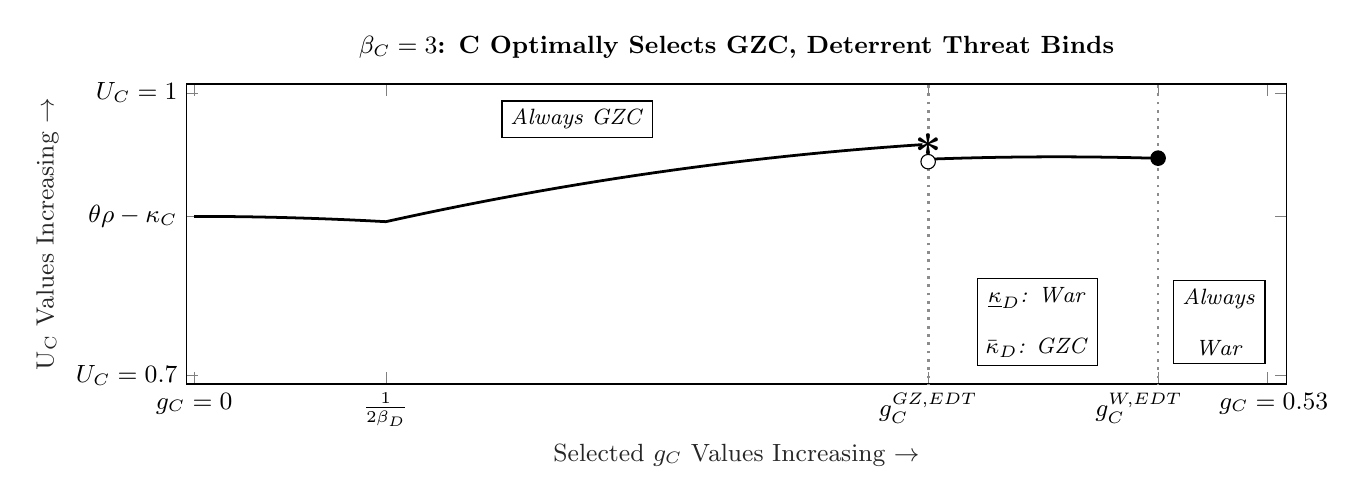
\begin{tikzpicture} 
\small
\begin{axis}[%
width=5.5in,
height=1.5in,
at={(1.011in,0.642in)},
scale only axis,
xmin=-0.004,
xmax=0.57,
xtick={0,0.1, 0.383,0.503,0.56},
xticklabels={{$g_C=0$},{$\frac{1}{2\beta_D}$},{$g_{C}^{GZ,EDT}$},{$g_{C}^{W,EDT}\,\,\,\,\,\,\,\,\,$},{$\,\,\,g_C=0.53$}},
xlabel style={font=\color{white!15!black}},
xlabel={Selected $g_C$ Values Increasing $\rightarrow$},
ymin=-.75,
ymax=.95,
ytick={-0.7,0.2,0.9},
yticklabels={{$U_C=0.7$},{$ \theta\rho-\kappa_C$},{$U_C=1$}},
ylabel style={font=\color{white!15!black}},
ylabel={$\text{U}_\text{C}$ Values Increasing $\rightarrow$},
axis background/.style={fill=white},
title style={font=\bfseries},
title={$\beta_C=3$: C Optimally Selects GZC, Deterrent Threat Binds},
]

\node[draw, align=center] at (0.2,0.75) {\footnotesize{\textit{Always GZC}}}; 
\node[draw, align=center] at (0.44,-0.4) {\footnotesize{\textit{$\underline{\kappa}_D$: War}} \\\footnotesize{\textit{$\bar{\kappa}_D$: GZC}}}; 
\node[draw, align=center] at (0.535,-0.4) {\footnotesize{\textit{Always}} \\\footnotesize{\textit{War}}}; 
\addplot [color=black, line width=1.0pt]
  table[row sep=crcr]{%
0	0.2	\\
0.01	0.1997	\\
0.02	0.1988	\\
0.03	0.1973	\\
0.04	0.1952	\\
0.05	0.1925	\\
0.06	0.1892	\\
0.07	0.1853	\\
0.08	0.1808	\\
0.09	0.1757	\\
0.1	0.17	\\
0.11	0.1937	\\
0.12	0.2168	\\
0.13	0.2393	\\
0.14	0.2612	\\
0.15	0.2825	\\
0.16	0.3032	\\
0.17	0.3233	\\
0.18	0.3428	\\
0.19	0.3617	\\
0.2	0.38	\\
0.21	0.3977	\\
0.22	0.4148	\\
0.23	0.4313	\\
0.24	0.4472	\\
0.25	0.4625	\\
0.26	0.4772	\\
0.27	0.4913	\\
0.28	0.5048	\\
0.29	0.5177	\\
0.3	0.53	\\
0.31	0.5417	\\
0.32	0.5528	\\
0.33	0.5633	\\
0.34	0.5732	\\
0.35	0.5825	\\
0.36	0.5912	\\
0.37	0.5993	\\
0.38	0.6068	\\
};

\addplot [color=black, line width=1.0pt]
  table[row sep=crcr]{%
0.385   0.524825 \\
0.39	0.5267	\\
0.4	0.53	\\
0.41	0.5327	\\
0.42	0.5348	\\
0.43	0.5363	\\
0.44	0.5372	\\
0.45	0.5375	\\
0.46	0.5372	\\
0.47	0.5363	\\
0.48	0.5348	\\
0.49	0.5327	\\
0.5	0.53	\\
};

\addplot [color=white!55!black, dotted, line width=1.0pt, forget plot]
  table[row sep=crcr]{%
0.383	-1\\
0.383	1\\
};

\addplot [color=white!55!black, dotted, line width=1.0pt, forget plot]
  table[row sep=crcr]{%
0.503	-1\\
0.503	1\\
};

\node at (0.383,0.57) {\LARGE \textbf{*}};
\node at (0.383,0.51) [circle,scale=0.6,draw,fill=black!0] {};
\node at (0.503,0.53) [circle,scale=0.6,minimum size=0.5pt,draw,fill=black!100] {};

\end{axis}
\end{tikzpicture} \vspace{.6cm}

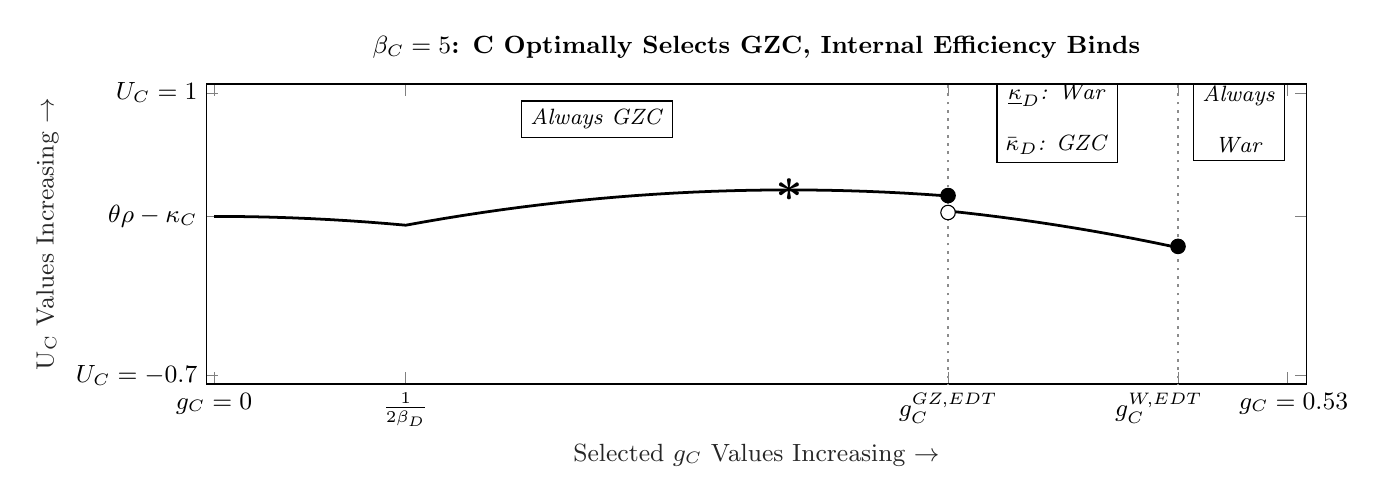
\begin{tikzpicture} 
\small
\begin{axis}[%
width=5.5in,
height=1.5in,
at={(1.011in,0.642in)},
scale only axis,
xmin=-0.004,
xmax=0.57,
xtick={0,0.1, 0.383,0.503,0.56},
xticklabels={{$g_C=0$},{$\frac{1}{2\beta_D}$},{$g_{C}^{GZ,EDT}$},{$g_{C}^{W,EDT}\,\,\,\,\,\,\,\,\,$},{$\,\,\,g_C=0.53$}},
xlabel style={font=\color{white!15!black}},
xlabel={Selected $g_C$ Values Increasing $\rightarrow$},
ymin=-.75,
ymax=.95,
ytick={-0.7,0.2,0.9},
yticklabels={{$U_C=-0.7$},{$ \theta\rho-\kappa_C$},{$U_C=1$}},
ylabel style={font=\color{white!15!black}},
ylabel={$\text{U}_\text{C}$ Values Increasing $\rightarrow$},
axis background/.style={fill=white},
title style={font=\bfseries},
title={$\beta_C=5$: C Optimally Selects GZC, Internal Efficiency Binds },
]

\node[draw, align=center] at (0.2,0.75) {\footnotesize{\textit{Always GZC}}}; 
\node[draw, align=center] at (0.44,0.75) {\footnotesize{\textit{$\underline{\kappa}_D$: War}} \\\footnotesize{\textit{$\bar{\kappa}_D$: GZC}}}; 
\node[draw, align=center] at (0.535,0.75) {\footnotesize{\textit{Always}} \\\footnotesize{\textit{War}}}; 
\addplot [color=black, line width=1.0pt]
  table[row sep=crcr]{%
0	0.2	\\
0.01	0.1995	\\
0.02	0.198	\\
0.03	0.1955	\\
0.04	0.192	\\
0.05	0.1875	\\
0.06	0.182	\\
0.07	0.1755	\\
0.08	0.168	\\
0.09	0.1595	\\
0.1	0.15	\\
0.11	0.1695	\\
0.12	0.188	\\
0.13	0.2055	\\
0.14	0.222	\\
0.15	0.2375	\\
0.16	0.252	\\
0.17	0.2655	\\
0.18	0.278	\\
0.19	0.2895	\\
0.2	0.3	\\
0.21	0.3095	\\
0.22	0.318	\\
0.23	0.3255	\\
0.24	0.332	\\
0.25	0.3375	\\
0.26	0.342	\\
0.27	0.3455	\\
0.28	0.348	\\
0.29	0.3495	\\
0.3	0.35	\\
0.31	0.3495	\\
0.32	0.348	\\
0.33	0.3455	\\
0.34	0.342	\\
0.35	0.3375	\\
0.36	0.332	\\
0.37	0.3255	\\
0.38	0.318	\\
};

\addplot [color=black, line width=1.0pt]
  table[row sep=crcr]{%
0.385	0.228	\\  
0.39	0.2225	\\
0.4	0.21	\\
0.41	0.1965	\\
0.42	0.182	\\
0.43	0.1665	\\
0.44	0.15	\\
0.45	0.1325	\\
0.46	0.114	\\
0.47	0.0945	\\
0.48	0.074	\\
0.49	0.0525	\\
0.5	0.03	\\
};

\addplot [color=white!55!black, dotted, line width=1.0pt, forget plot]
  table[row sep=crcr]{%
0.383	-1\\
0.383	1\\
};

\addplot [color=white!55!black, dotted, line width=1.0pt, forget plot]
  table[row sep=crcr]{%
0.503	-1\\
0.503	1\\
};

\node at (0.3, 0.31) {\LARGE \textbf{*}};
\node at (0.383,0.222) [circle,scale=0.6,draw,fill=black!0] {};
\node at (0.383,0.318) [circle,scale=0.6,minimum size=0.5pt,draw,fill=black!100] {};
\node at (0.503,0.03) [circle,scale=0.6,minimum size=0.5pt,draw,fill=black!100] {};
            
\end{axis}
\end{tikzpicture}\vspace{.6cm}

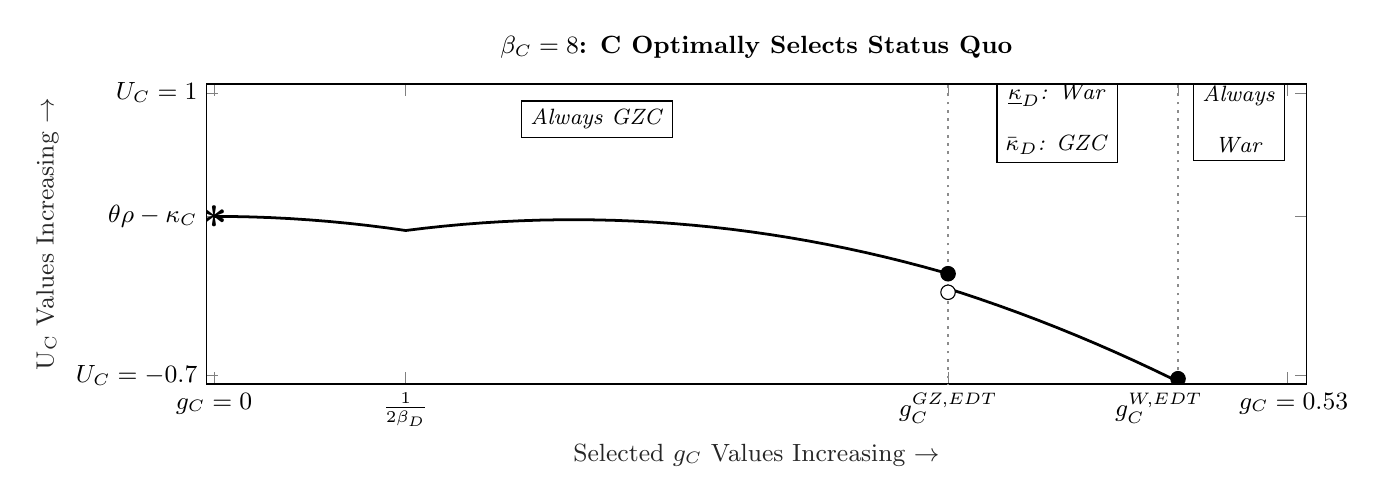
\begin{tikzpicture} 
\small
\begin{axis}[%
width=5.5in,
height=1.5in,
at={(1.011in,0.642in)},
scale only axis,
xmin=-0.004,
xmax=0.57,
xtick={0,0.1, 0.383,0.503,0.56},
xticklabels={{$g_C=0$},{$\frac{1}{2\beta_D}$},{$g_{C}^{GZ,EDT}$},{$g_{C}^{W,EDT}\,\,\,\,\,\,\,\,\,$},{$\,\,\,g_C=0.53$}},
xlabel style={font=\color{white!15!black}},
xlabel={Selected $g_C$ Values Increasing $\rightarrow$},
ymin=-.75,
ymax=.95,
ytick={-0.7,0.2,0.9},
yticklabels={{$U_C=-0.7$},{$ \theta\rho-\kappa_C$},{$U_C=1$}},
ylabel style={font=\color{white!15!black}},
ylabel={$\text{U}_\text{C}$ Values Increasing $\rightarrow$},
axis background/.style={fill=white},
title style={font=\bfseries},
title={$\beta_C=8$: C Optimally Selects Status Quo},
]

\node[draw, align=center] at (0.2,0.75) {\footnotesize{\textit{Always GZC}}}; 
\node[draw, align=center] at (0.44,0.75) {\footnotesize{\textit{$\underline{\kappa}_D$: War}} \\\footnotesize{\textit{$\bar{\kappa}_D$: GZC}}}; 

\node[draw, align=center] at (0.535,0.75) {\footnotesize{\textit{Always}} \\\footnotesize{\textit{War}}}; 
\addplot [color=black, line width=1.0pt]
  table[row sep=crcr]{%
0	0.2	\\
0.01	0.1992	\\
0.02	0.1968	\\
0.03	0.1928	\\
0.04	0.1872	\\
0.05	0.18	\\
0.06	0.1712	\\
0.07	0.1608	\\
0.08	0.1488	\\
0.09	0.1352	\\
0.1	0.12	\\
0.11	0.1332	\\
0.12	0.1448	\\
0.13	0.1548	\\
0.14	0.1632	\\
0.15	0.17	\\
0.16	0.1752	\\
0.17	0.1788	\\
0.18	0.1808	\\
0.19	0.1812	\\
0.2	0.18	\\
0.21	0.1772	\\
0.22	0.1728	\\
0.23	0.1668	\\
0.24	0.1592	\\
0.25	0.15	\\
0.26	0.1392	\\
0.27	0.1268	\\
0.28	0.1128	\\
0.29	0.0972	\\
0.3	0.08	\\
0.31	0.0612	\\
0.32	0.0408	\\
0.33	0.0188	\\
0.34	-0.0048	\\
0.35	-0.03	\\
0.36	-0.0568	\\
0.37	-0.0852	\\
0.38	-0.1152	\\
};

\addplot [color=black, line width=1.0pt]
  table[row sep=crcr]{%
0.385   -0.216 \\
0.39	-0.2338	\\
0.4	-0.27	\\
0.41	-0.3078	\\
0.42	-0.3472	\\
0.43	-0.3882	\\
0.44	-0.4308	\\
0.45	-0.475	\\
0.46	-0.5208	\\
0.47	-0.5682	\\
0.48	-0.6172	\\
0.49	-0.6678	\\
0.5	-0.72	\\
};

\addplot [color=white!55!black, dotted, line width=1.0pt, forget plot]
  table[row sep=crcr]{%
0.383	-1\\
0.383	1\\
};

\addplot [color=white!55!black, dotted, line width=1.0pt, forget plot]
  table[row sep=crcr]{%
0.503	-1\\
0.503	1\\
};

\node at (0,0.16) {\LARGE \textbf{*}};
\node at (0.383,-.23) [circle,scale=0.6,draw,fill=black!0] {};
\node at (0.383,-0.125) [circle,scale=0.6,minimum size=0.5pt,draw,fill=black!100] {};
\node at (0.503,-0.72) [circle,scale=0.6,minimum size=0.5pt,draw,fill=black!100] {};
          
\end{axis}
\end{tikzpicture}

\caption{C's Utility Across selected $g_C$'s (Status Quo \& Gray Zone Conflict Outcomes).}\label{constraints1}
\caption*{ C's optimal $g_C$ is marked by the asterisks. The regions denote how D responds to a selected $g_C$---whether D will always engage with a gray zone response, whether D will always go to war, or whether different types of D respond differently. All sub-figures have the same underlying parameters (listed in the Appendix), except $\beta_C$ which varies across sub-figures.}
\end{figure}

First consider the top panel within Figure \ref{constraints1} (with the title ``$\beta_{C}=3$: C Optimally Selects GZC, Deterrent Threat Binds''). For a fixed set of parameters,\footnote{The parameters for all figures are listed in the Appendix.} this figure displays C selecting some $g_{C}$ on the x-axis, and C's final expected payoff given D's and C's best responses following C's choice of $g_C$ on the y-axis. C's equilibrium  selection, $g_C^*$, is denoted by the asterisks. 

In the top panel, when $g_{C}=0$, C selects into the status quo, and D neither wants to go to war ($w_{D}^*=0$) nor wants to implement any costly response ($g_{D}^{*}=0$). Later in the game, D makes an offer that gives C their wartime utility, and C will accept. 

When $g_{C}\in(0,\frac{1}{2\beta_{D}}]$, C's utility is decreasing in $g_{C}$. For any $g_{C}$ in this region, D will optimally respond with a gray zone response at level $g_{D}^{*}=min\left\{ g_{C},\frac{1}{2\beta_{D}}\right\}$, which effectively cancels out the benefits of C's challenge. And, because C is still paying costs for conducting the challenge, C does worse if C chooses to select greater challenges within this region.

When $g_{C}\in(\frac{1}{2\beta_{D}},g_{C}^{GZ,EDT}]$, C's utility is increasing in $g_{C}$. Here, D's limited response ($g_{D}^{*}=\frac{1}{2\beta_{D}})$ is not enough to cancel out C's challenge, which means C's challenges start being productive. And, while C is facing costs to implementing more aggressive challenges, here $\beta_{C}$ is not high enough to prevent C's utility from increasing (under these parameters, $g_{C}^{GZ,EDT}<g_{C}^{GZ,IE}$).

Moving to the right of $g_{C}=g_{C}^{GZ,EDT}$, different types of D begin to play the game differently, which creates a discontinuity. Type $\underline{\kappa}_{D}$ D will go to war for any $g_{C}$ to the right of the threshold. And, type $\bar{\kappa}_{D}$ D (who is worse at war) is still willing to tolerate challenges slightly beyond $g_{C}^{GZ,EDT}$. Together, C's utility has a discontinuity because C is now going to war with probability $\omega$, which is bad for C, and because C is not gaining much from small increases in $g_{C}$ against type $\bar{\kappa}_{D}$. When $g_{C}\in(g_{C}^{GZ,EDT},g_{C}^{W,EDT}]$, C's utility is increasing in $g_{C}$. So long that C's costs to $g_{C}$ are low enough (as they are here: $g_{C}^{W,EDT}<g_{C}^{W,IE}$), C will do better selecting more aggressive challenges, as this will result in C doing better against type $\bar{\kappa}_{D}$.

Finally, there is another discontinuity at $g_{C}^{W,EDT}$, and for any $g_{C}>g_{C}^{W,EDT}$ C's utility is low and decreasing in $g_{C}$. Here both types of D will go to war, which is bad for C. Additionally, C incurs the costs of conducting the challenge while still ending up fighting a war with both types of D. Overall, these payoffs are (literally) off-the-chart bad, and for all parameters C prefers selecting into the status quo to any $g_{C}$ in this space. Under this set of parameters, C attains the greatest utility by selecting $g_{C}^{*}=g_{C}^{GZ,EDT}$. Verbally, here C is willing to conduct the greatest challenge that will not push either type of D into war, resulting in an outcome of gray zone conflict.

Now consider the middle panel in Figure \ref{constraints1} (with the title ``$\beta_{C}=5$: C Optimally Selects GZC, Internal Efficiency Binds''), where all parameters are the same except $\beta_{C}=5$. Here C's costs of challenging have gone up, which alters the slopes of how $g_C$ relates to C's payoffs. Now $g_{C}^{GZ,EDT}\geq g_{C}^{GZ,IE}$ holds, meaning C's internal efficiency constraint binds, and now C selects a challenge based on their own internal costs and benefits of challenging. Instead of C selecting the most aggressive challenge they can that will not push D to declare war, C now does best stopping short of this value, instead selecting $g_{C}^{*}=g_{C}^{GZ,IE}$. Finally, in the bottom panel, we increase $\beta_C$ again and fix $\beta_{C}=8$. Here C's costs of challenging have increased so much that it is never productive for C to engage in any challenge, and C prefers selecting into the status quo.

Figure \ref{constraints2} considers a different set of parameters and illustrates other possible equilibria to the game. In the top panel (titled ``$\beta_{C}=1.8$: C Optimally Risks War, Deterrent Threat Binds''), C does best setting $g_{C}^{*}=g_{C}^{W,EDT}$. Even though by selecting $g_{C}^{*}=g_{C}^{W,EDT}$ C must fight if D is type $\underline{\kappa}_{D}$, which is bad for C, C is undertaking a more aggressive challenge against type $\bar{\kappa}_{D}$, which is good for C. Together, C's expected payoff from taking a more aggressive challenge and risking war is greater than C's expected payoff from never risking war ($g_{C}=g_{C}^{GZ,EDT}$) or selecting into the status quo ($g_{C}=0$). Finally, in the bottom panel of Figure \ref{constraints2}, C faces slightly greater costs to challenging (all parameters are the same except now $\beta_{C}=2.5$), which results in inequality $g_{C}^{W,EDT}\geq g_{C}^{W,IE}$ holding; this means C will not select the greatest $g_{C}$ possible that will keep type $\bar{\kappa}_{D}$ from declaring war, but will rather scale back their selected challenge due to their internal efficiency constraint.

\begin{figure}  

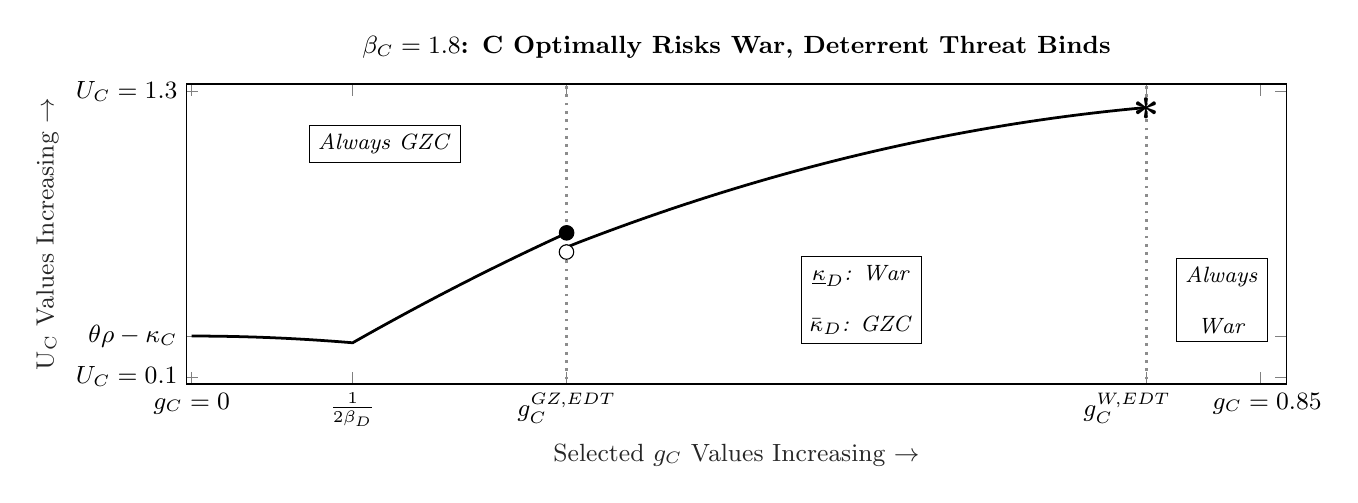
\begin{tikzpicture} 
\small
\begin{axis}[%
width=5.5in,
height=1.5in,
at={(1.011in,0.642in)},
scale only axis,
xmin=-0.004,
xmax=0.85,
xtick={0,0.125, 0.2911,0.7411,0.83},
xticklabels={{$g_C=0$},{$\frac{1}{2\beta_D}$},{$g_{C}^{GZ,EDT}$},{$g_{C}^{W,EDT}\,\,\,\,\,\,\,\,\,$},{$\,\,\,g_C=0.85$}},
xlabel style={font=\color{white!15!black}},
xlabel={Selected $g_C$ Values Increasing $\rightarrow$},
ymin=0.05,
ymax=1.3,
ytick={0.08,0.25,1.27},
yticklabels={{$U_C=0.1$},{$ \theta\rho-\kappa_C$},{$U_C=1.3$}},
ylabel style={font=\color{white!15!black}},
ylabel={$\text{U}_\text{C}$ Values Increasing $\rightarrow$},
axis background/.style={fill=white},
title style={font=\bfseries},
title={$\beta_C=1.8$: C Optimally Risks War, Deterrent Threat Binds},
]

\node[draw, align=center] at (0.15,1.05) {\footnotesize{\textit{Always GZC}}}; 

\node[draw, align=center] at (0.52,0.4) {\footnotesize{\textit{$\underline{\kappa}_D$: War}} \\\footnotesize{\textit{$\bar{\kappa}_D$: GZC}}}; 

\node[draw, align=center] at (0.8,.4) {\footnotesize{\textit{Always}} \\\footnotesize{\textit{War}}}; 


\addplot [color=black, line width=1.0pt]
  table[row sep=crcr]{%
0	0.25	\\
0.01	0.24982	\\
0.02	0.24928	\\
0.03	0.24838	\\
0.04	0.24712	\\
0.05	0.2455	\\
0.06	0.24352	\\
0.07	0.24118	\\
0.08	0.23848	\\
0.09	0.23542	\\
0.1	0.232	\\
0.11	0.22822	\\
0.1125	0.22721875	\\
0.115	0.226195	\\
0.1175	0.22514875	\\
0.12	0.22408	\\
0.1225	0.22298875	\\
0.125	0.221875	\\
0.1275	0.22948875	\\
0.13	0.23708	\\
0.1325	0.24464875	\\
0.135	0.252195	\\
0.1375	0.25971875	\\
0.14	0.26722	\\
0.1425	0.27469875	\\
0.145	0.282155	\\
0.1475	0.28958875	\\
0.15	0.297	\\
0.16	0.32642	\\
0.17	0.35548	\\
0.18	0.38418	\\
0.19	0.41252	\\
0.2	0.4405	\\
0.21	0.46812	\\
0.22	0.49538	\\
0.23	0.52228	\\
0.24	0.54882	\\
0.25	0.575	\\
0.26	0.60082	\\
0.27	0.62628	\\
0.28	0.65138	\\
0.29	0.67612	\\
};


\addplot [color=black, line width=1.0pt]
  table[row sep=crcr]{%
0.2911 0.62 \\
0.3	0.63925	\\
0.31	0.65977	\\
0.32	0.67993	\\
0.33	0.69973	\\
0.34	0.71917	\\
0.35	0.73825	\\
0.36	0.75697	\\
0.37	0.77533	\\
0.38	0.79333	\\
0.39	0.81097	\\
0.4	0.82825	\\
0.41	0.84517	\\
0.42	0.86173	\\
0.43	0.87793	\\
0.44	0.89377	\\
0.45	0.90925	\\
0.46	0.92437	\\
0.47	0.93913	\\
0.48	0.95353	\\
0.49	0.96757	\\
0.5	0.98125	\\
0.51	0.99457	\\
0.52	1.00753	\\
0.53	1.02013	\\
0.54	1.03237	\\
0.55	1.04425	\\
0.56	1.05577	\\
0.57	1.06693	\\
0.58	1.07773	\\
0.59	1.08817	\\
0.6	1.09825	\\
0.61	1.10797	\\
0.62	1.11733	\\
0.63	1.12633	\\
0.64	1.13497	\\
0.65	1.14325	\\
0.66	1.15117	\\
0.67	1.15873	\\
0.68	1.16593	\\
0.69	1.17277	\\
0.7	1.17925	\\
0.71	1.18537	\\
0.72	1.19113	\\
0.73	1.19653	\\
0.74	1.20157	\\
};




%\addplot [color=white!55!black, dotted, line width=1.0pt, forget plot]
%  table[row sep=crcr]{%
%0.1	-1\\
%0.1	1\\
%};


\addplot [color=white!55!black, dotted, line width=1.0pt, forget plot]
  table[row sep=crcr]{%
0.2911	0\\
0.2911	1.5\\
};

\addplot [color=white!55!black, dotted, line width=1.0pt, forget plot]
  table[row sep=crcr]{%
0.741	0\\
0.741	1.5\\
};


\node at (0.741,1.17) {\LARGE \textbf{*}};
\node at (0.291,0.6) [circle,scale=0.6,draw,fill=black!0] {};
\node at (0.2911,0.68) [circle,scale=0.6,minimum size=0.5pt,draw,fill=black!100] {};
%\node at (0.503,0.53) [circle,scale=0.6,minimum size=0.5pt,draw,fill=black!100] {};
            


\end{axis}
\end{tikzpicture} \vspace{.6cm}

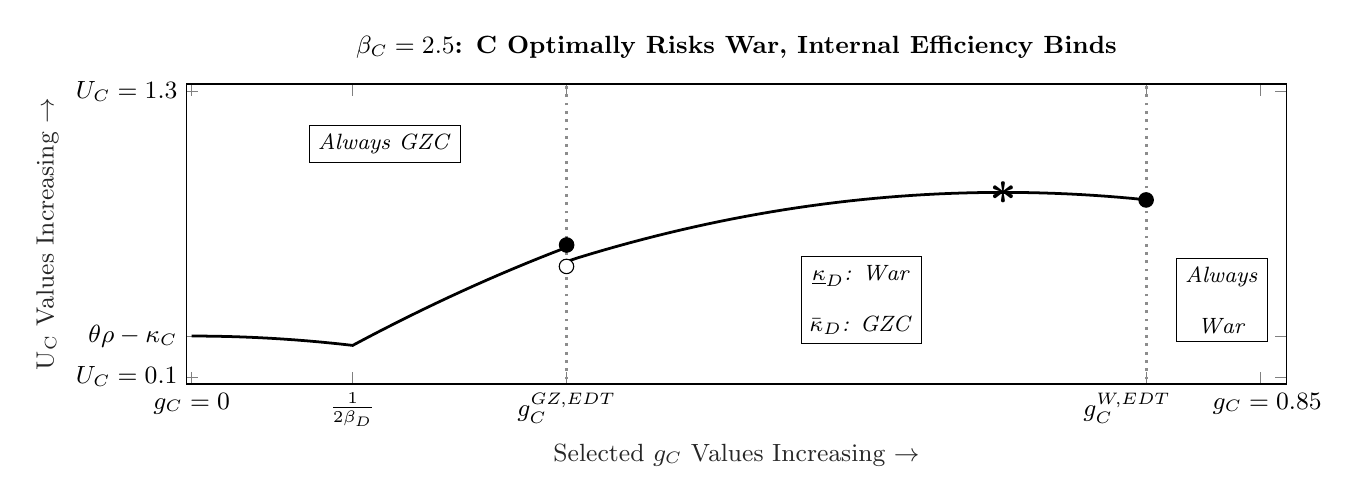
\begin{tikzpicture} 
\small
\begin{axis}[%
width=5.5in,
height=1.5in,
at={(1.011in,0.642in)},
scale only axis,
xmin=-0.004,
xmax=0.85,
xtick={0,0.125, 0.2911,0.7411,0.83},
xticklabels={{$g_C=0$},{$\frac{1}{2\beta_D}$},{$g_{C}^{GZ,EDT}$},{$g_{C}^{W,EDT}\,\,\,\,\,\,\,\,\,$},{$\,\,\,g_C=0.85$}},
xlabel style={font=\color{white!15!black}},
xlabel={Selected $g_C$ Values Increasing $\rightarrow$},
ymin=0.05,
ymax=1.3,
ytick={0.08,0.25,1.27},
yticklabels={{$U_C=0.1$},{$ \theta\rho-\kappa_C$},{$U_C=1.3$}},
ylabel style={font=\color{white!15!black}},
ylabel={$\text{U}_\text{C}$ Values Increasing $\rightarrow$},
axis background/.style={fill=white},
title style={font=\bfseries},
title={$\beta_C=2.5$: C Optimally Risks War, Internal Efficiency Binds},
]

\node[draw, align=center] at (0.15,1.05) {\footnotesize{\textit{Always GZC}}}; 

\node[draw, align=center] at (0.52,0.4) {\footnotesize{\textit{$\underline{\kappa}_D$: War}} \\\footnotesize{\textit{$\bar{\kappa}_D$: GZC}}}; 

\node[draw, align=center] at (0.8,.4) {\footnotesize{\textit{Always}} \\\footnotesize{\textit{War}}}; 


\addplot [color=black, line width=1.0pt]
  table[row sep=crcr]{%
0	0.25	\\
0.01	0.24975	\\
0.02	0.249	\\
0.03	0.24775	\\
0.04	0.246	\\
0.05	0.24375	\\
0.06	0.241	\\
0.07	0.23775	\\
0.08	0.234	\\
0.09	0.22975	\\
0.1	0.225	\\
0.11	0.21975	\\
0.1125	0.218359375	\\
0.115	0.2169375	\\
0.1175	0.215484375	\\
0.12	0.214	\\
0.1225	0.212484375	\\
0.125	0.2109375	\\
0.1275	0.218109375	\\
0.13	0.22525	\\
0.1325	0.232359375	\\
0.135	0.2394375	\\
0.1375	0.246484375	\\
0.14	0.2535	\\
0.1425	0.260484375	\\
0.145	0.2674375	\\
0.1475	0.274359375	\\
0.15	0.28125	\\
0.16	0.3085	\\
0.17	0.33525	\\
0.18	0.3615	\\
0.19	0.38725	\\
0.2	0.4125	\\
0.21	0.43725	\\
0.22	0.4615	\\
0.23	0.48525	\\
0.24	0.5085	\\
0.25	0.53125	\\
0.26	0.5535	\\
0.27	0.57525	\\
0.28	0.5965	\\
0.29	0.61725	\\
};


\addplot [color=black, line width=1.0pt]
  table[row sep=crcr]{%
0.291	0.56	\\
0.3	0.57625	\\
0.31	0.5925	\\
0.32	0.60825	\\
0.33	0.6235	\\
0.34	0.63825	\\
0.35	0.6525	\\
0.36	0.66625	\\
0.37	0.6795	\\
0.38	0.69225	\\
0.39	0.7045	\\
0.4	0.71625	\\
0.41	0.7275	\\
0.42	0.73825	\\
0.43	0.7485	\\
0.44	0.75825	\\
0.45	0.7675	\\
0.46	0.77625	\\
0.47	0.7845	\\
0.48	0.79225	\\
0.49	0.7995	\\
0.5	0.80625	\\
0.51	0.8125	\\
0.52	0.81825	\\
0.53	0.8235	\\
0.54	0.82825	\\
0.55	0.8325	\\
0.56	0.83625	\\
0.57	0.8395	\\
0.58	0.84225	\\
0.59	0.8445	\\
0.6	0.84625	\\
0.61	0.8475	\\
0.62	0.84825	\\
0.63	0.8485	\\
0.64	0.84825	\\
0.65	0.8475	\\
0.66	0.84625	\\
0.67	0.8445	\\
0.68	0.84225	\\
0.69	0.8395	\\
0.7	0.83625	\\
0.71	0.8325	\\
0.72	0.82825	\\
0.73	0.8235	\\
0.74	0.81825	\\
};




%\addplot [color=white!55!black, dotted, line width=1.0pt, forget plot]
%  table[row sep=crcr]{%
%0.1	-1\\
%0.1	1\\
%};


\addplot [color=white!55!black, dotted, line width=1.0pt, forget plot]
  table[row sep=crcr]{%
0.2911	0\\
0.2911	1.5\\
};

\addplot [color=white!55!black, dotted, line width=1.0pt, forget plot]
  table[row sep=crcr]{%
0.741	0\\
0.741	1.5\\
};


\node at (0.63,0.82) {\LARGE \textbf{*}};
\node at (0.291,0.54) [circle,scale=0.6,draw,fill=black!0] {};
\node at (0.2911,0.6294) [circle,scale=0.6,minimum size=0.5pt,draw,fill=black!100] {};
\node at (0.741,0.817) [circle,scale=0.6,minimum size=0.5pt,draw,fill=black!100] {};
            


\end{axis}
\end{tikzpicture}


\caption{C's Utility Across selected $g_C$'s (War Outcomes).}\label{constraints2}
\caption*{ C's optimal $g_C$ is marked by the asterisks. The regions denote how D responds to a selected $g_C$---whether D will always engage with a gray zone response, whether D will always go to war, or whether  different types of D respond differently. All sub-figures have the same underlying parameters (listed in the Appendix), except $\beta_C$ which varies across sub-figures.}
\end{figure}

\subsection{Statement of Equilibrium}

The equilibrium is as follows.

\textbf{Stage 5:} If $x\geq P(g_{C},g_{D})-\frac{\kappa_{C}}{\theta}$, then C sets $w_{C}=0$. Otherwise, C sets $w_{C}=1$. If C previously set $g_{C}=min\left\{ \frac{1}{4\beta_{D}}+\bar{\kappa}_{D}+\frac{\kappa_{C}}{\theta},\frac{(1-\omega)\theta}{2\beta_{C}}\right\} $, then C believes D is type $\bar{\kappa}_{D}$ with probability $1$. Otherwise, C believes D is type $\bar{\kappa}_{D}$ ($\underline{\kappa}_{D}$) with probability $1-\omega$ ($\omega$).

\textbf{Stage 4:} D always sets $x=P(g_{C},g_{D})-\frac{\kappa_{C}}{\theta}.$

\textbf{Stage 3:} For $\kappa_{D}\in\{\underline{\kappa}_{D},\bar{\kappa}_{D}\}$, if $1-P(0,0)-\kappa_{D}>1-P(g_{C},min\left\{ \frac{1}{2\beta_{D}},g_{C}\right\} )+\frac{\kappa_{C}}{\theta}-\beta_{D}*\left(min\left\{ \frac{1}{2\beta_{D}},g_{C}\right\} \right)^{2}$, then D will set $w_{D}=1$. Otherwise, D will set $w_{D}=0$ and $g_{D}=min\left\{ \frac{1}{2\beta_{D}},g_{C}\right\}.$

\textbf{Stage 2:} C believes D is type $\bar{\kappa}_{D}$ with probability $1-\omega$ and type $\underline{\kappa}_{D}$ with probability $\omega$. C's selection of a challenge is as follows:

\textit{Sometimes War, Deterrent Threat Binds:} C sets %$g_{C}=g_{C}^{W,EDT}=\frac{1}{4\beta_{D}}+\bar{\kappa}_{D}+\frac{\kappa_{C}}{\theta}$ 
$g_{C}=g_{C}^{W,EDT}$ 
if $g_{C}^{W,IE}>g_{C}^{W,EDT}$, $\omega\left(\theta\rho-\kappa_{C}\right)+(1-\omega)\theta\left(\rho-\frac{1}{4\beta_{D}}+\bar{\kappa}_{D}\right)-\beta_{C}\left(g_{C}^{W,EDT}\right)^{2}>\theta\rho-\kappa_{C}$, and $\omega\left(\theta\rho-\kappa_{C}\right)+(1-\omega)\theta\left(\rho-\frac{1}{4\beta_{D}}+\bar{\kappa}_{D}\right)-\beta_{C}\left(g_{C}^{W,EDT}\right)^{2}>\theta\left(\rho-\frac{1}{4\beta_{D}}+\underline{\kappa}_{D}\right)-\beta_{C}\left(g_{C}^{GZ,EDT}\right)^{2}$.

\textit{Sometimes War, Internal Efficiency Binds:} C sets
$g_{C}=g_{C}^{W,IE}$
%$g_{C}=g_{C}^{W,IE}=\frac{(1-\omega)\theta}{2\beta_{C}}$ 
if $g_{C}^{W,IE}>g_{C}^{GZ,EDT}$, $g_{C}^{W,IE}\le g_{C}^{W,EDT}$, $\omega\left(\theta\rho-\kappa_{C}\right)+(1-\omega)\left(\theta\rho+\frac{(1-\omega)\theta^{2}}{2\beta_{C}}-\frac{\theta}{2\beta_{D}}-\kappa_{C}\right)-\beta_{C}\left(g_{C}^{W,IE}\right)^{2}>\theta\rho-\kappa_{C}$, and $\omega\left(\theta\rho-\kappa_{C}\right)+(1-\omega)\left(\theta\rho+\frac{(1-\omega)\theta^{2}}{2\beta_{C}}-\frac{\theta}{2\beta_{D}}-\kappa_{C}\right)-\beta_{C}\left(g_{C}^{W,IE}\right)^{2}>\theta\left(\rho-\frac{1}{4\beta_{D}}+\underline{\kappa}_{D}\right)-\beta_{C}\left(g_{C}^{GZ,EDT}\right)^{2}$.

\textit{Always Gray Zone, Deterrent Threat Binds:}\textbf{ }C sets
$g_{C}=g_{C}^{GZ,EDT}$
%$g_{C}=g_{C}^{GZ,EDT}=\frac{1}{4\beta_{D}}+\underline{\kappa}_{D}+\frac{\kappa_{C}}{\theta}$\textbf{ }
if $\theta\rho-\kappa_{C}<\theta\left(\rho-\frac{1}{4\beta_{D}}+\underline{\kappa}_{D}\right)-\beta_{C}\left(g_{C}^{GZ,EDT}\right)^{2}$ and any of the following holds: (a)\textbf{ }$g_{C}^{GZ,IE}>g_{C}^{GZ,EDT}$ and $g_{C}^{W,IE}\le g_{C}^{GZ,EDT}$ ; (b) $g_{C}^{W,IE}>g_{C}^{GZ,EDT}$, $g_{C}^{W,IE}\le g_{C}^{W,EDT},$ and $\theta\left(\rho-\frac{1}{4\beta_{D}}+\underline{\kappa}_{D}\right)-\beta_{C}\left(g_{C}^{GZ,EDT}\right)^{2}\geq\omega\left(\theta\rho-\kappa_{C}\right)+(1-\omega)\left(\theta\rho+\frac{(1-\omega)\theta^{2}}{2\beta_{C}}-\frac{\theta}{2\beta_{D}}-\kappa_{C}\right)-\beta_{C}\left(g_{C}^{W,IE}\right)^{2}$; or (c) $g_{C}^{W,IE}>g_{C}^{W,EDT}$, and $\theta\left(\rho-\frac{1}{4\beta_{D}}+\underline{\kappa}_{D}\right)-\beta_{C}\left(g_{C}^{GZ,EDT}\right)^{2}\geq\omega\left(\theta\rho-\kappa_{C}\right)+(1-\omega)\theta\left(\rho-\frac{1}{4\beta_{D}}+\bar{\kappa}_{D}\right)-\beta_{C}\left(g_{C}^{W,EDT}\right)^{2}$.

\textit{Always Gray Zone, Internal Efficiency Binds:} C sets 
$g_{C}=g_{C}^{GZ,IE}$
%$g_{C}=g_{C}^{GZ,IE}=\frac{\theta}{2\beta_{C}}$ 
if 
$g_{C}^{GZ,IE}\leq g_{C}^{GZ,EDT}$ and $\theta\rho-\kappa_{C}<\theta\rho+\frac{\theta^{2}}{4\beta_{C}}-\frac{\theta}{2\beta_{D}}-\kappa_{C}$.

\textit{Status Quo}: C sets $g_{C}=0$ if any of the following holds: (a) $g_{C}^{GZ,IE}\leq g_{C}^{GZ,EDT}$ and $\theta\rho-\kappa_{C}\geq\theta\rho+\frac{\theta^{2}}{4\beta_{C}}-\frac{\theta}{2\beta_{D}}-\kappa_{C}$; (b) $g_{C}^{GZ,IE}>g_{C}^{GZ,EDT}$, $g_{C}^{W,IE}\leq g_{C}^{GZ,EDT}$, and $\theta\rho-\kappa_{C}\geq\theta\left(\rho-\frac{1}{4\beta_{D}}+\underline{\kappa}_{D}\right)-\beta_{C}\left(g_{C}^{GZ,EDT}\right)^{2}$; (c) $g_{C}^{W,IE}>g_{C}^{GZ,EDT}$, $g_{C}^{W,IE}\le g_{C}^{W,EDT},$$\theta\rho-\kappa_{C}\geq\theta\left(\rho-\frac{1}{4\beta_{D}}+\underline{\kappa}_{D}\right)-\beta_{C}\left(g_{C}^{GZ,EDT}\right)^{2}$, and $\theta\rho-\kappa_{C}\geq\omega\left(\theta\rho-\kappa_{C}\right)+(1-\omega)\left(\theta\rho+\frac{(1-\omega)\theta^{2}}{2\beta_{C}}-\frac{\theta}{2\beta_{D}}-\kappa_{C}\right)-\beta_{C}\left(g_{C}^{W,IE}\right)^{2}$; or (d) $g_{C}^{W,IE}>g_{C}^{W,EDT},$$\theta\rho-\kappa_{C}\geq\theta\left(\rho-\frac{1}{4\beta_{D}}+\underline{\kappa}_{D}\right)-\beta_{C}\left(g_{C}^{GZ,EDT}\right)^{2}$, and $\theta\rho-\kappa_{C}\geq\omega\left(\theta\rho-\kappa_{C}\right)+(1-\omega)\theta\left(\rho-\frac{1}{4\beta_{D}}+\bar{\kappa}_{D}\right)-\beta_{C}\left(g_{C}^{W,EDT}\right)^{2}$.

We discuss the equilibrium conditions in detail in the Appendix Section 1.3.

\section{What Drives Variation in Gray Zone Activity?} \label{useme}

Our model and its equilibrium are consistent with gray zone conflict being multifaceted, but add value by establishing two underlying, rational mechanisms for how challengers conduct gray zone conflict. First, the challenger may select their challenges based on the external deterrent threat, essentially pulling their punches in gray zone conflict to avoid a risk of war. Second, when the external deterrent threat does not bind, the challenger selects their challenge based on their own internal efficiency, essentially choosing their optimal challenge unconstrained by the risk of further escalation. Those who claim that Russia (or any other state engaging in gray zone conflict) conducts whatever kind of gray zone conflict they want and operates outside the realm of standard deterrence dynamics are describing a challenger behaving based on their internal efficiency constraint. However, it could also be that Russia is limiting their challenges in order to avoid a greater escalation---which is more consistent with the external deterrent threat binding.

Here we establish how observable patterns can distinguish whether the challenger's behavior is shaped by their internal efficiency or their external deterrent threat. This allows us to use the relationships uncovered by statistical analysis to suggest whether our challenger is behaving based on the logic of deterrence, or not. To be clear, these are not Observations describing a test of the model; rather, the statistical analysis in the next section is done to identify empirical patterns, which is then used as fodder for our theory \citep{hoover_methodologyeconometrics_2006, clarke_modeldisciplinepolitical_2012}. 
Put another way, in this Section,  we provide a roadmap for how to use empirical findings that we can estimate to uncover the internal motivations for how challengers behave (i.e. what constraint binds).

\subsection{On the Defender's Willingness to go to War and Conflict Intensity}
The observed relationship between the defender's willingness to go to war, here approximated by $\kappa$, and the challenger's selected challenges, $g_{C}^{*}$, depends on whether the challenger's internal efficiency or the defender's external deterrent threat shapes the challenger's decision making.

When the external deterrent threat binds, the defender's willingness to escalate to war creates an upper bound on the tolerated level of the selected challenge. If we observe a challenger decreasing their challenges as a defender becomes more willing to go to war, then we know that the challenger's decisions are influenced by deterrence. For example, suppose under one set of parameters the challenger wants to select a challenge that will avoid war and where the external deterrent threat binds (formally $g_{C}^{*}=g_{C}^{GZ,EDT}=\frac{1}{4\beta_{D}}+\underline{\kappa}_{D}+\frac{\kappa_{C}}{\theta}$). If the defender becomes more willing to go to war and the challenger wishes to continue avoiding war, then the challenger becomes restricted in what challenges they can implement. This can play out in one of two ways. First, the challenger could continue selecting the challenge level that results in gray zone conflict ($g_{C}^{*}=g_{C}^{GZ,EDT}$), meaning, as $\kappa$ decreases, the challenger must decrease their challenge.\footnote{Put another way, $g_{C}^{GZ,EDT}(\kappa)$ is decreasing in its argument.} Second, as the defender becomes more willing to go to war, the challenger could switch from selecting a challenge that results in gray zone conflict ($g_{C}^{*}=g_{C}^{GZ,EDT}$) to not challenging in the first place ($g_{C}^{*}=0$). Together, when the challenger is responding to the external deterrent threat and is facing a defender that is more willing to fight, the challenger will pursue less aggressive challenges. 

When the internal efficiency constraint binds, the challenger's costs and resolve determine the selected challenge. If we observe a challenger not altering their challenges as a defender becomes more willing to go to war, then we know the challenger is not responding to the defender's external threat from war, but rather is basing their decisions on their internal cost-benefit calculations. For example, suppose the challenger is selecting a challenge that will always result in gray zone conflict and where the internal efficiency constraint binds (formally $g_{C}^{*}=g_{C}^{GZ,IE}=\frac{\theta}{2\beta_{C}}$). If $\kappa$ then decreases, as long as the internal efficiency constraint continues to bind, then there will be no changes in the selected $g_{C}^{*}$. Put another way, when the challenger is acting based on their internal efficiency and facing a defender that is more willing to fight, the challenger is non-reactive. Of course, it could also be that as $\kappa$ decreases, the internal efficiency constraint no longer binds, and the external efficiency constraint starts to bind. When this is the case, the logic in the previous paragraph applies.

Consider Figure \ref{fig:optimaldetdecrease}, which illustrates the dynamics described above. On the x-axis, left-to-right, the defender's deterrent threat from war is increasing ($\kappa$ is decreasing). On the y-axis, we plot the challenger's selected equilibrium challenge $g_{C}^{*}$. For the greatest costs of war (the greatest $\kappa$), the challenger is unconstrained by the defender's external deterrent threat. This means that the challenger can freely select their challenge based on their internal cost-benefit balancing. Thus, the defender's costs of war do not play a role in the challenger's decision making here. Moving to the right (to the second region), the defender gets better at war, and the challenger cannot conduct the same level of challenge without provoking the defender. Here, the external deterrent threat starts to bind, and, to remain in gray zone conflict, the challenger must scale back their challenge, which results in $g_{C}^{*}$ decreasing. Moving to the right further (to the third region), the defender is very willing to fight. Here the challenger is so constrained in what challenges they can conduct that will still result in gray zone conflict that the challenger no longer finds gray zone conflict to be productive. Under these very low values of $\kappa$, the challenger will select into the status quo ($g_C^*=0$).

Altogether, Figure \ref{fig:optimaldetdecrease} illustrates a natural intuition. As the defender's deterrent threat from war increases, the challenger cannot select as aggressive of challenges without provoking the defender to war. Decreasing $\kappa$ results in a lower intensity of gray zone conflict until the challenger no longer finds gray zone conflict worthwhile.

\begin{figure}[h]
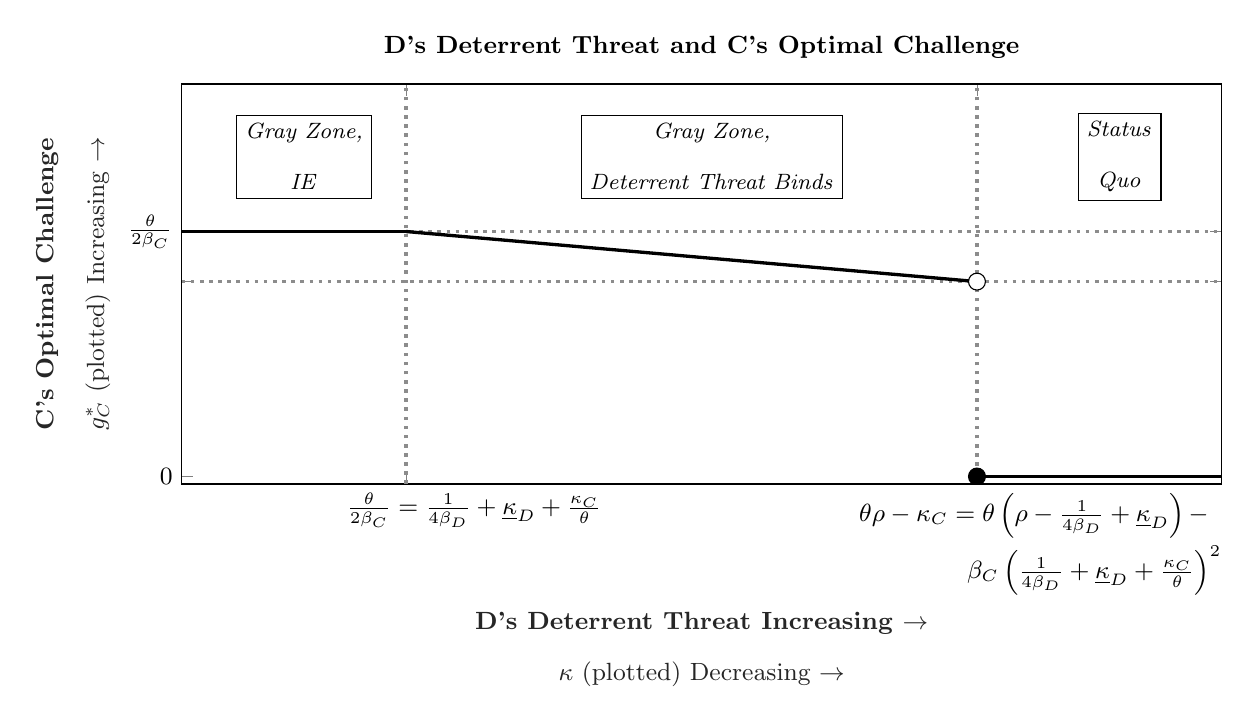
\begin{tikzpicture} 
    \small
    \begin{axis}[%
    width=5.2in,
    height=2in,
    at={(1.011in,0.642in)},
    scale only axis,
    xmin=-0.5,
    xmax=-0.245,
    xtick={-0.5, -0.445, -0.305, -.245},
    xticklabels={{},
    {\;\;\;\;\;\;\;\;\;\;\;\;\;\;\;\;\;\; $\frac{\theta}{2\beta_{C}}=\frac{1}{4\beta_{D}}+\underline{\kappa}_{D}+\frac{\kappa_{C}}{\theta}$},
    {\shortstack{$\;\;\;\;\;\;\;\;\;\;\;\;\;\;\;\; \theta\rho-\kappa_{C}=\theta\left(\rho-\frac{1}{4\beta_{D}}+\underline{\kappa}_{D}\right)-$\\$\;\;\;\;\;\;\;\;\;\;\;\;\;\;\;\;\;\;\;\;\;\;\;\;\;\;\;\;\;\;\;\;\; \beta_{C}\left(\frac{1}{4\beta_{D}}+\underline{\kappa}_{D}+\frac{\kappa_{C}}{\theta}\right)^{2}$}},
    {}},
    xlabel style={font=\color{white!15!black},align=center},
    xlabel={\textbf{D's Deterrent Threat Increasing $\rightarrow$} \\ $\kappa$ (plotted) Decreasing $\rightarrow$ },
    ymin=0,
    ymax=1.1,
    ytick={0.02,0.5567,0.69444},
    yticklabels={{0},
%    {\shortstack{{}\\{}\\($\rho_{W}-\rho_{0}+$\\$\underline{\kappa_{D}}+\frac{1}{4\beta_{D}}$)}},
    {},
    {$\frac{\theta}{2\beta_C}$}},
    ylabel style={font=\color{white!15!black}, align=center},
    ylabel={\textbf{C's Optimal Challenge} \\ $g_{C}^*$ (plotted) Increasing $\rightarrow$},
    axis background/.style={fill=white},
    title style={font=\bfseries},
    title={D's Deterrent Threat and C's Optimal Challenge},
    ]
    
    \node[draw, align=center] at (-0.27,.9) {\footnotesize{\textit{Status}}\\ \footnotesize{\textit{Quo}}};
    
    \node[draw, align=center] at (-0.37,0.9) {\footnotesize{\textit{Gray Zone,}} \\ \footnotesize{\textit{Deterrent Threat Binds}}}; 
    \node[draw, align=center] at (-.47,0.9) {\footnotesize{\textit{Gray Zone,}} \\ \footnotesize{\textit{IE}}};

    \addplot [color=white!55!black, dotted, line width=1.3pt, forget plot]
      table[row sep=crcr]{%
    -0.445	0\\
    -0.445	1.5\\
    };
    \addplot [color=white!55!black, dotted, line width=1.3pt, forget plot]
      table[row sep=crcr]{%
    -0.305	0\\
    -0.305	1.5\\
    };
    
    \addplot [color=white!55!black, dotted, line width=1.3pt, forget plot]
      table[row sep=crcr]{%
    -0.5 	0.5567\\
    0	0.5567\\
    };
    \addplot [color=white!55!black, dotted, line width=1.3pt, forget plot]
      table[row sep=crcr]{%
    -0.5 	0.69444\\
    0	0.69444\\
    };

    \addplot [color=black, line width=1.2pt]
      table[row sep=crcr]{%
    -0.5		0.69444	\\
    -0.445		0.69444\\
    };

    \addplot [color=black, line width=1.2pt]
      table[row sep=crcr]{%
    -0.445		0.69444	\\
    -0.305		0.556666667\\
    };

    \addplot [color=black, line width=1.2pt, forget plot]
      table[row sep=crcr]{%
    -0.305	0.02	\\
    -.245		0.02	\\
    };

        \node at (-0.305,0.0207)  [circle,scale=0.7,minimum size=0.5pt,draw,fill=black!100] {};
        \node at (-0.305,0.556666667)  [circle,scale=0.7,draw,fill=black!0] {};

    \end{axis}
    \end{tikzpicture} \caption{C's Optimal Challenge as D's Deterrent Threat Decreases.}
\caption*{C's selected challenge under a range of $\kappa$'s are plotted. \textquotedblleft Gray Zone, IE\textquotedblright{} describes the equilibrium space where the outcome will always be gray zone conflict and C's internal efficiency constraint binds. The first vertical boundary---where $\frac{\theta}{2\beta_{C}}=\frac{1}{4\beta_{D}}+\underline{\kappa}_{D}+\frac{\kappa_{C}}{\theta}$---defines where $\kappa$ has increased to the cutpoint where D's deterrent threat will start to constrain C's gray zone behavior. The second horizontal boundary---where $\theta\rho-\kappa_{C}=\theta\left(\rho-\frac{1}{4\beta_{D}}+\underline{\kappa}_{D}\right)-\beta_{C}\left(\frac{1}{4\beta_{D}}+\underline{\kappa}_{D}+\frac{\kappa_{C}}{\theta}\right)^{2}$---is the cutpoint where D's external constraint is so strong that C prefers accepting the status quo to engaging in gray zone conflict.}
\label{fig:optimaldetdecrease}
\end{figure}

Two other dynamics are worth discussing. First, under the parameters in Figure \ref{fig:optimaldetdecrease}, when $\kappa$ decreases enough, the challenger switched into the status quo. Under different parameters, as $\kappa$ decreases, the challenger may similarly feel constrained within gray zone conflict, but may switch to sometimes risking war.\footnote{Formally, when C conducts gray zone conflict and is constrained by the external deterrent threat, C will select $g_{C}^{*}=\frac{1}{4\beta_{D}}+\underline{\kappa}_{D}+\frac{\kappa_{C}}{\theta}$. As the defender becomes better at war, the challenger will either opt into the status quo and set $g_{C}^{*}=0$, or select a greater challenge and risk war by setting $g_{C}^{*}=min\left\{ \frac{(1-\omega)\theta}{2\beta_{C}},\frac{1}{4\beta_{D}}+\bar{\kappa}_{D}+\frac{\kappa_{C}}{\theta}\right\} $. %As an example, fix parameters $\rho=0.1$, $\kappa_{C}=0.1$, $\psi=0.1$, $\beta_{D}=1.5$, $\beta_{C}=0.8$, $\theta=1.23$, and $\omega=0.1$. As $\kappa$ decreases from $\kappa=0.5$ to $\kappa=.25$, C will switch from always playing the game to end in gray zone conflict and begin risking war.
} What distinguishes these cases is the challenger's willingness to fight. When the challenger responds to increases in the defender's willingness to go to war by scaling back their challenge to nothing, the challenger is clearly deterred. When the challenger responds to increases in the defender's willingness to go to war by engaging in more aggressive and riskier behavior, the defender's deterrent threat is not constraining the challenger, and we will say the challenger is choosing their challenge based on their internal efficiency.

Second, a similar dynamic can play out when the challenger begins by sometimes risking war. If the external deterrent threat constraint binds and $\kappa$ decreases, C will either decreased their challenge (still selecting $g_{C}^{*}=g_{C}^{W,EDT}$, which is decreasing in $\kappa$), or revert to selecting into the status quo ($g_{C}^{*}=0$). Alternatively, if the challenger sometimes risks war, the challenger's internal efficiency constraint binds, and $\kappa$ decreases, then C will be non-responsive until $\kappa$ decreases enough so that the external deterrent threat constraint binds. 

How the challenger's responds to changes in $\kappa$ can be summarized in Observations 1 and 2. 

\textbf{\textit{Observation 1:}}\textit{ If increasing the defender's willingness to go to war (decreasing $\kappa$) results in the challenger decreasing their selected challenge ($g_{C}$), then the external deterrent threat shapes the challenger's selected challenge.}

\textbf{\textit{Observation 2:}}\textit{ If increasing the defender's willingness to go to war results in the challenger not changing their selected challenge, increasing their selected challenge, or risking war more, then the challenger's internal efficiency shapes the challenger's selected challenge.}

These Observations (and Observations 3-6 below) are not describing ``tests'' of the model. Rather, these Observations describe how, if we observe specific empirical patterns in the data, we can back out whether external deterrence or the challenger's internal optimization is driving the challenger's behavior. For example, Observation 1 suggests that if we observe a positive relationship between $\kappa$ and $g_{C}^{*}$, then deterrence is playing a role in shaping the challenger's behavior. This Observation uses the comparative statics from the model to bridge what can be observed empirically to what motivates the scope of an actor's gray zone conflict levels.

\subsection{On the Challenger's Resolve and Conflict Intensity}

When the internal efficiency constraint binds, the challenger selects their challenges based on how much they care about the asset and how costly it is to engage in more aggressive challenges. If we observe decreased challenges over issues that the challenger cares less about (approximated by a lower $\theta$), then we know the challenger's decisions are based on their internal efficiency calculations. For example, suppose under one set of parameters the challenger will select a challenge that sometimes risks war and where the internal efficiency constraint binds ($g_{C}^{*}=g_{C}^{W,IE}=\frac{(1-\omega)\theta}{2\beta_{C}}$). As the challenger's resolve ($\theta$) decreases, the challenger will limit their selected challenge in one of several different ways. First, the challenger may continue to risk war, but will select a more conservative challenge (i.e. still select $g_{C}^{*}=g_{C}^{W,IE}$, but this value is smaller). Alternatively, the challenger may no longer find it worthwhile to risk war and may switch into a more conservative challenge that always result in gray zone conflict ($g_{C}^{*}=g_{C}^{GZ,IE}$ or $g_{C}^{*}=g_{C}^{GZ,EDT}$). Finally, if the challenger's resolve decreases enough, the challenger no longer finds it worthwhile to challenge and will accept the status quo ($g_{C}^{*}=0$). Together, when the challenger is responding to their internal efficiency, as the challenger's resolve decreases, the challenger will pursue less aggressive challenges.

If we observe less aggressive challenges over issues that challengers care more about, then we know the challenger's decisions are influenced by deterrence (and vice-versa). This (counter-intuitive) relationship stems from the bargaining component of the game. As the challenger's resolve increases, the defender must offer the challenger a greater policy concession in the fourth stage to avoid the challenger declaring war in the fifth stage.\footnote{In equilibrium, $x=P(g_{C},g_{D})-\frac{\kappa_{C}}{\theta}.$} This greater concession in Stage 4 constrains how aggressive the challenge can be without triggering the defender to go to war in Stage 3. Specifically, whenever the deterrent threat binds, the challenger scales back their challenge, knowing they will be compensated later for doing so.\footnote{This is formally captured in $g_{C}^{GZ,EDT}=\frac{1}{4\beta_{D}}+\underline{\kappa}_{D}+\frac{\kappa_{C}}{\theta}$ and $g_{C}^{W,EDT}=\frac{1}{4\beta_{D}}+\bar{\kappa}_{D}+\frac{\kappa_{C}}{\theta}$} For this reason, whenever the challenger is responding to the external deterrent threat, as the challenger's resolve decreases, the challenger will pursue more aggressive challenges. 

We illustrate these dynamics in Figure \ref{fig:optimalresolveincrease}. When C has a sufficiently low resolve (sufficiently low $\theta$), C will not challenge and will accept the status quo. Moving to the right, as the challenger values the asset more, the challenger eventually begins engaging in challenges. Within the next equilibrium space (GZ, IE), the challenger's challenges are not aggressive enough to reach the defender's threshold for declaring war; this means that the internal efficiency constraint binds, and the challenge is increasing in the challenger's resolve. The selected challenge increases in $\theta$ until the challenger becomes constrained by the defender's willingness to go to war, or when the defender's deterrent threat binds (Gray Zone, EDT).\footnote{This switch happens when $\frac{1}{4\beta_{D}}+\underline{\kappa}_{D}+\frac{\kappa_{C}}{\theta}$ becomes smaller than $\frac{\theta}{2\beta_{C}}.$} Within this region, as discussed above, the challenger's optimal challenge is decreasing in $\theta$. Then eventually, the challenger's resolve increases to the cutpoint where the challenger becomes willing to risk war with the privately-good-at-war types of the defender in order to conduct a greater challenge against the privately-bad-at-war types. This is where war sometimes occurs, and there is a similar relationship between the challenger's internal efficiency (War, IE) and defender's deterrent threat (War, EDT). 

\begin{figure}[h]
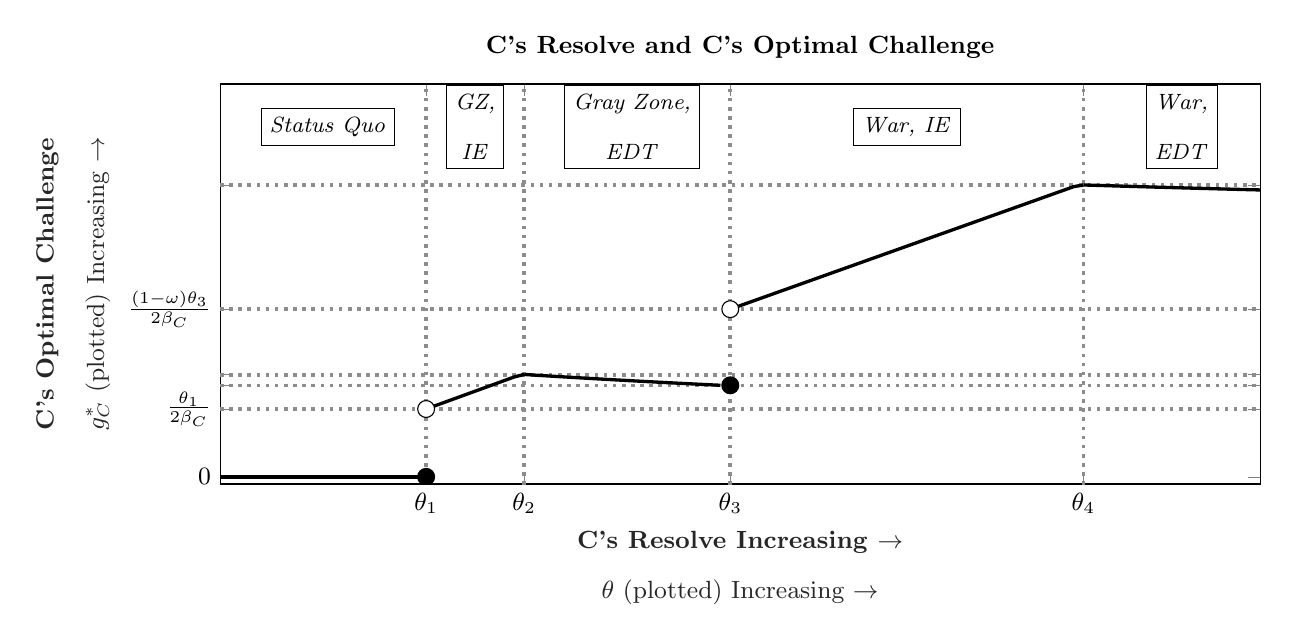
\begin{tikzpicture} 
    \small
    \begin{axis}[%
    width=5.2in,
    height=2in,
    at={(1.011in,0.642in)},
    scale only axis,
    xmin=1,
    xmax=2.06,
    xtick={1.21,1.31,1.52,1.88},
    xticklabels={
    {$\theta_1$},
    {$\theta_2$},
    {$\theta_3$},
    {$\theta_4$},
    {}
    },
    xlabel style={font=\color{white!15!black},align=center},
    xlabel={\textbf{C's Resolve Increasing $\rightarrow$} \\ $\theta$ (plotted) Increasing $\rightarrow$},
    ymin=0.5,
    ymax=1.06,
    ytick={0.51,0.605, 0.653, 0.6382, 0.7448, 0.9187},
    yticklabels={{0},
    {$\frac{\theta_1}{2\beta_{C}}$},
    %{$\frac{1}{4\beta_{D}}+\underline{\kappa}_{D}+\frac{\kappa_{C}}{\theta}$},
    {},
    {},
    {$\frac{(1-\omega)\theta_3}{2\beta_{C}}$},
    {}
    },
    ylabel style={font=\color{white!15!black}, align=center},
    ylabel={\textbf{C's Optimal Challenge} \\ $g_{C}^*$ (plotted) Increasing $\rightarrow$},
    axis background/.style={fill=white},
    title style={font=\bfseries},
    title={C's Resolve and C's Optimal Challenge},
    ]
    
    \node[draw, align=center] at (1.11,1) {\footnotesize{\textit{Status Quo}}};
    \node[draw, align=center] at (1.26,1) {\footnotesize{\textit{GZ,}} \\ \footnotesize{\textit{IE}}}; 
    \node[draw, align=center] at (1.42,1) {\footnotesize{\textit{Gray Zone,}} \\ \footnotesize{\textit{EDT}}}; 
    \node[draw, align=center] at (1.7,1) {\footnotesize{\textit{War, IE}}};
    \node[draw, align=center] at (1.98,1) {\footnotesize{\textit{War,}} \\ \footnotesize{\textit{EDT}}};

    %BEGIN DOTTED LINES
    \addplot [color=white!55!black, dotted, line width=1.3pt, forget plot]
      table[row sep=crcr]{%
    1.21	0\\
    1.21	1.5\\
    };
    \addplot [color=white!55!black, dotted, line width=1.3pt, forget plot]
      table[row sep=crcr]{%
    1.31	0\\
    1.31	1.5\\
    };
    
    \addplot [color=white!55!black, dotted, line width=1.3pt, forget plot]
      table[row sep=crcr]{%
    1.52	0\\
    1.52	1.5\\
    };

     \addplot [color=white!55!black, dotted, line width=1.3pt, forget plot]
      table[row sep=crcr]{%
    1.88	0\\
    1.88	1.5\\
    };
    \addplot [color=white!55!black, dotted, line width=1.3pt, forget plot]
      table[row sep=crcr]{%
    1 	0.605\\
    3	0.605\\
    };

    \addplot [color=white!55!black, dotted, line width=1.3pt, forget plot]
      table[row sep=crcr]{%
    1 	0.653\\
    3	0.653\\
    };
      \addplot [color=white!55!black, dotted, line width=1.3pt, forget plot]
      table[row sep=crcr]{%
    1 	0.6382\\
    3	0.6382\\
    };
    
       \addplot [color=white!55!black, dotted, line width=1.3pt, forget plot]
      table[row sep=crcr]{%
    1 	0.7448\\
    3	0.7448\\
    };
 
        \addplot [color=white!55!black, dotted, line width=1.3pt, forget plot]
      table[row sep=crcr]{%
    1 	0.9187\\
    3	0.9187\\
    };
 
        \addplot [color=black, line width=1.2pt]
      table[row sep=crcr]{%
    1 	0.51\\
    1.21	0.51\\
    };

    \addplot [color=black, line width=1.2pt]
      table[row sep=crcr]{%
    1.21	0.605	\\
1.22	0.61	\\
1.23	0.615	\\
1.24	0.62	\\
1.25	0.625	\\
1.26	0.63	\\
1.27	0.635	\\
1.28	0.64	\\
1.29	0.645	\\
1.3	0.65	\\
1.31	0.653392706	\\
    };

    \addplot [color=black, line width=1.2pt]
      table[row sep=crcr]{%
1.31	0.653392706	\\
1.32	0.652525253	\\
1.33	0.651670844	\\
1.34	0.650829187	\\
1.35	0.65	\\
1.36	0.649183007	\\
1.37	0.64837794	\\
1.38	0.647584541	\\
1.39	0.646802558	\\
1.4	0.646031746	\\
1.41	0.645271868	\\
1.42	0.644522692	\\
1.43	0.643783994	\\
1.44	0.643055556	\\
1.45	0.642337165	\\
1.46	0.641628615	\\
1.47	0.640929705	\\
1.48	0.64024024	\\
1.49	0.63956003	\\
1.5	0.638888889	\\
1.51	0.638226637	\\
    };

    \addplot [color=black, line width=1.2pt]
      table[row sep=crcr]{%
1.52	0.7448	\\
1.53	0.7497	\\
1.54	0.7546	\\
1.55	0.7595	\\
1.56	0.7644	\\
1.57	0.7693	\\
1.58	0.7742	\\
1.59	0.7791	\\
1.6	0.784	\\
1.61	0.7889	\\
1.62	0.7938	\\
1.63	0.7987	\\
1.64	0.8036	\\
1.65	0.8085	\\
1.66	0.8134	\\
1.67	0.8183	\\
1.68	0.8232	\\
1.69	0.8281	\\
1.7	0.833	\\
1.71	0.8379	\\
1.72	0.8428	\\
1.73	0.8477	\\
1.74	0.8526	\\
1.75	0.8575	\\
1.76	0.8624	\\
1.77	0.8673	\\
1.78	0.8722	\\
1.79	0.8771	\\
1.8	0.882	\\
1.81	0.8869	\\
1.82	0.8918	\\
1.83	0.8967	\\
1.84	0.9016	\\
1.85	0.9065	\\
1.86	0.9114	\\
1.87	0.9163	\\
1.88	0.918676123	\\
    };

    \addplot [color=black, line width=1.2pt]
      table[row sep=crcr]{%
1.88	0.918676123	\\
1.89	0.918253968	\\
1.9	0.917836257	\\
1.91	0.91742292	\\
1.92	0.917013889	\\
1.93	0.916609096	\\
1.94	0.916208477	\\
1.95	0.915811966	\\
1.96	0.915419501	\\
1.97	0.915031021	\\
1.98	0.914646465	\\
1.99	0.914265773	\\
2	0.913888889	\\
2.01	0.913515755	\\
2.02	0.913146315	\\
2.03	0.912780515	\\
2.04	0.912418301	\\
2.05	0.912059621	\\
2.06	0.911704423	\\
    };
    
  \node at (1.21,0.51)  [circle,scale=0.7,minimum size=0.5pt,draw,fill=black!100] {};
  \node at (1.21,0.605)  [circle,scale=0.7,draw,fill=black!0] {};
    
       \node at (1.52,0.6382)  [circle,scale=0.7,minimum size=0.5pt,draw,fill=black!100] {};
        \node at (1.52,0.7448)  [circle,scale=0.7,draw,fill=black!0] {}; 

    \end{axis}
    \end{tikzpicture} \caption{Optimal Challenge as C's Resolve Increases.}
\caption*{C's optimal challenge intensity under a range of $\theta$'s. %We abbreviate ``gray zone'' with ``GZ,'' the ``internal efficiency constraint binds'' with ``IE,'' and the external ``deterrent threat binds'' with ``EDT.''
 $\theta_{1}$ is the value of $\theta$ where $\theta_{1}\rho-\kappa_{C}=\theta_{1}\rho+\frac{\theta_{1}^{2}}{4\beta_{C}}-\frac{\theta_{1}}{2\beta_{D}}-\kappa_{C}$, or C's gray zone payoffs are equal to C selecting into the status quo. $\theta_{2}$ is where $\frac{\theta_{2}}{2\beta_{C}}=\frac{1}{4\beta_{D}}+\underline{\kappa}_{D}+\frac{\kappa_{C}}{\theta_{2}}$, or where, within gray zone conflict, C's internal efficiency constraint is equal to the D's deterrent threat constraint. $\theta_{3}$ is where $\theta_{3}\left(\rho-\frac{1}{4\beta_{D}}+\underline{\kappa}_{D}\right)-\beta_{C}\left(\frac{1}{4\beta_{D}}+\underline{\kappa}_{D}+\frac{\kappa_{C}}{\theta_{3}}\right)^{2}=(1-\omega)\left(\theta_{3}\rho+\frac{(1-\omega)\theta_{3}^{2}}{2\beta_{C}}-\frac{\theta_{3}}{2\beta_{D}}-\kappa_{C}\right)+\omega\left(\theta_{3}\rho-\kappa_{C}\right)-\beta_{C}\left(\frac{(1-\omega)\theta_{3}}{2\beta_{C}}\right)^{2}$, or where C is indifferent between selecting into gray zone conflict and sometimes risking war. $\theta_{4}$ is where $\frac{(1-\omega)\theta_{4}}{2\beta_{C}}=\frac{1}{4\beta_{D}}+\bar{\kappa}_{D}+\frac{\kappa_{C}}{\theta_{4}}$, or where, within cases where C sometime risks war, C's internal efficiency constraint is equal to the D's deterrent threat constraint. %To simplify labeling, the y-axis is not drawn to scale.
}
\label{fig:optimalresolveincrease}
\end{figure}

How the challenger's responds to changes in $\theta$ is summarized in Observations 3 and 4.

\textbf{\textit{Observation 3:}}\textit{ If increasing the challenger's resolve ($\theta$) results in the challenger increasing their selected challenge, then the challenger's internal efficiency shapes the challenger's selected challenge. }

\textbf{\textit{Observation 4:}}\textit{ If increasing the challenger's resolve results in the challenger decreasing their selected challenge, then the external deterrent threat shapes the challenger's selected challenge.}

\subsection{On the Challenger's Gray Zone Costs and Conflict Intensity}

When the internal efficiency constraint binds, the challenger bases their challenges on how much they care about the asset and how costly it is to engage in more aggressive challenges. If we observe less aggressive challenges as the challenger's costs increases (approximated by greater $\beta_{C}$), then we know the challenger's decisions are based on their internal efficiency. In contrast, when the external deterrent threat constraint binds, the challenger bases their challenges on the defender's willingness to go to war, which is independent of C's internal costs to challenging. If we observe no change in the selected challenges as the challenger's costs are increasing, then we know the challenger's decisions are based on the external deterrent threat.

Across all equilibria, as the challenger's challenge costs decrease ($\beta_{C}$ decreases), the challenger will select weakly more aggressive challenges ($g_{C}^{*}$). Figure \ref{fig:optimalcostvary} illustrates one example this. We do not discuss these results at length because these findings are relatively straightforward. How the challenger's responds to changes in $\beta_C$ can be summarized in Observations 5 and 6.

\begin{figure}[h]
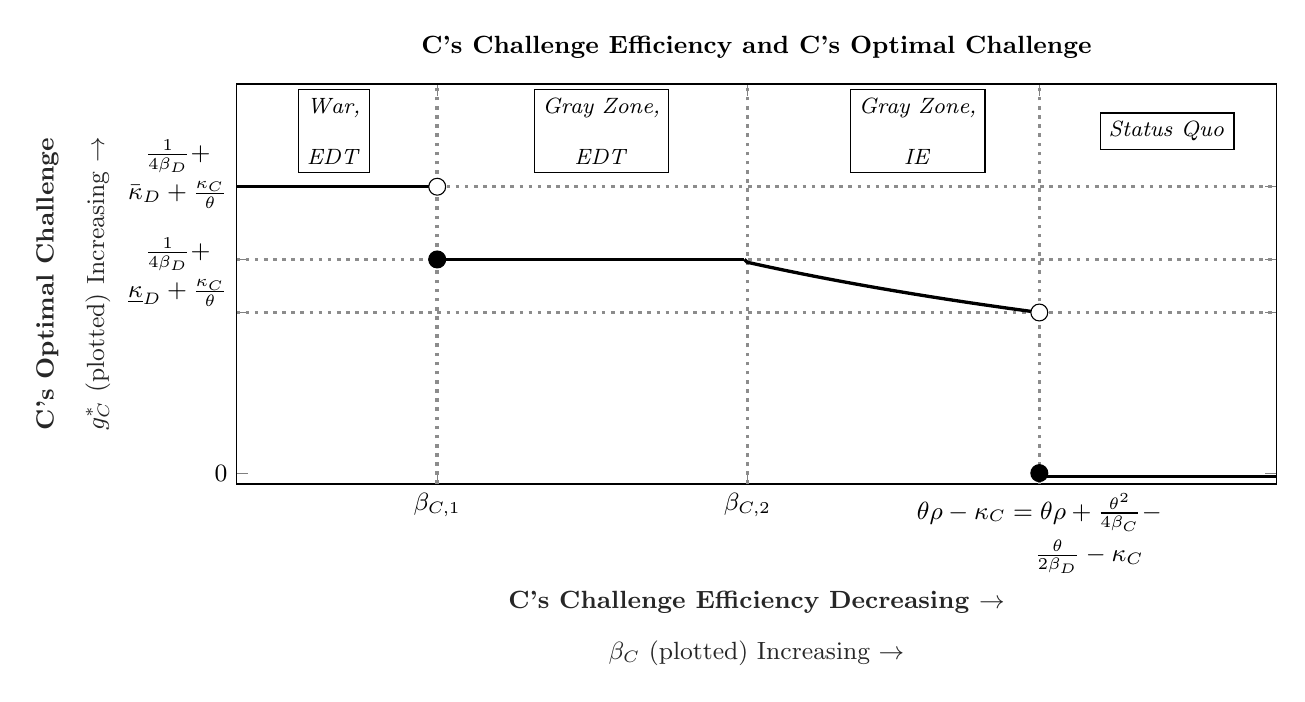
\begin{tikzpicture} 
    \small
    \begin{axis}[%
    width=5.2in,
    height=2in,
    at={(1.011in,0.642in)},
    scale only axis,
    xmin=0.8,
    xmax=2.51,
    xtick={0.8, 1.13, 1.64, 2.12},
    xticklabels={{},
    {$\beta_{C,1}$},
    {$\beta_{C,2}$},
    {\shortstack{$\theta\rho-\kappa_{C}=\theta\rho+\frac{\theta^{2}}{4\beta_{C}}-$\\$\;\;\;\;\;\;\;\;\;\;\;\;\;\; \frac{\theta}{2\beta_{D}}-\kappa_{C}$}}},
    xlabel style={font=\color{white!15!black},align=center},
    xlabel={\textbf{C's Challenge Efficiency Decreasing $\rightarrow$} \\ $\beta_C$ (plotted) Increasing $\rightarrow$ },
    ymin=0,
    ymax=1.1,
    ytick={0.03, 0.472, 0.6176,0.818},
    yticklabels={{0},
    {},
    %{\shortstack{{}\\{}\\($\rho_{W}-\rho_{0}+$\\$\kappa_{D}+\frac{1}{4\beta_D}$)}}
    {\shortstack{{\color{white}A}\\{$\frac{1}{4\beta_{D}}+$}\\{$\underline{\kappa}_{D}+\frac{\kappa_{C}}{\theta}$}}},
    {\shortstack{{$\frac{1}{4\beta_{D}}+$}\\{$\bar{\kappa}_{D}+\frac{\kappa_{C}}{\theta}$}\\{\color{white}A}}}
    },
    ylabel style={font=\color{white!15!black}, align=center},
    ylabel={\textbf{C's Optimal Challenge} \\ $g_{C}^*$ (plotted) Increasing $\rightarrow$},
    axis background/.style={fill=white},
    title style={font=\bfseries},
    title={C's Challenge Efficiency and C's Optimal Challenge},
    ]
    
        \addplot [color=white!55!black, dotted, line width=1.3pt, forget plot]
      table[row sep=crcr]{%
    1.13	0\\
    1.13	1.5\\
    };
    \addplot [color=white!55!black, dotted, line width=1.3pt, forget plot]
      table[row sep=crcr]{%
   1.64	0\\
    1.64	1.5\\
    };
    
        \addplot [color=white!55!black, dotted, line width=1.3pt, forget plot]
      table[row sep=crcr]{%
   2.12	0\\
    2.12	1.5\\
    };
    
    \addplot [color=white!55!black, dotted, line width=1.3pt, forget plot]
      table[row sep=crcr]{%
    0.8 	0.472\\
    3	0.472\\
    };
    
        \addplot [color=white!55!black, dotted, line width=1.3pt, forget plot]
      table[row sep=crcr]{%
    0.8 	0.6176\\
    3	0.6176\\
    };
    
        \addplot [color=white!55!black, dotted, line width=1.3pt, forget plot]
      table[row sep=crcr]{%
    0.8 	0.818\\
    3	0.818\\
    };
 
    \node[draw, align=center] at (0.96,0.97) {\footnotesize{\textit{War,}}\\ \footnotesize{\textit{EDT}}}; 
    \node[draw, align=center] at (1.4,.97) {\footnotesize{\textit{Gray Zone,}}\\ \footnotesize{\textit{EDT}}}; 
    
    \node[draw, align=center] at (1.92,.97) {\footnotesize{\textit{Gray Zone,}} \\ \footnotesize{\textit{IE}}};
    
        \node[draw, align=center] at (2.33,.97) {\footnotesize{\textit{Status Quo}}};

    \addplot [color=black, line width=1.2pt]
      table[row sep=crcr]{%
0.8	0.817567568	\\
0.83	0.817567568	\\
0.86	0.817567568	\\
0.89	0.817567568	\\
0.92	0.817567568	\\
0.95	0.817567568	\\
0.98	0.817567568	\\
1.01	0.817567568	\\
1.04	0.817567568	\\
1.07	0.817567568	\\
1.1	0.817567568	\\
1.13	0.817567568	\\
    };

    \addplot [color=black, line width=1.2pt]
      table[row sep=crcr]{%
 1.13	0.617567568	\\
1.19	0.617567568	\\
1.22	0.617567568	\\
1.25	0.617567568	\\
1.28	0.617567568	\\
1.31	0.617567568	\\
1.34	0.617567568	\\
1.37	0.617567568	\\
1.4	0.617567568	\\
1.43	0.617567568	\\
1.46	0.617567568	\\
1.49	0.617567568	\\
1.52	0.617567568	\\
1.55	0.617567568	\\
1.58	0.617567568	\\
1.61	0.617567568	\\
1.635	0.617567568	\\
    };

    \addplot [color=black, line width=1.2pt]
      table[row sep=crcr]{%
1.635	0.617567568	\\
1.64	0.609756098	\\
1.67	0.598802395	\\
1.7	0.588235294	\\
1.73	0.578034682	\\
1.76	0.568181818	\\
1.79	0.558659218	\\
1.82	0.549450549	\\
1.85	0.540540541	\\
1.88	0.531914894	\\
1.91	0.523560209	\\
1.94	0.515463918	\\
1.97	0.507614213	\\
2	0.5	\\
2.03	0.492610837	\\
2.06	0.485436893	\\
2.09	0.4784689	\\
2.12	0.471698113	\\
    };
    
    \addplot [color=black, line width=1.2pt, forget plot]
      table[row sep=crcr]{%
    2.12	0.02	\\
    2.51	0.02	\\
    };

        \node at ( 1.13,	0.617567568) [circle,scale=0.7,minimum size=0.5pt,draw,fill=black!100] {};
        \node at  (1.13,	0.817567568)   [circle,scale=0.7,draw,fill=black!0] {};
    
 
         \node at ( 2.12,		0.03) [circle,scale=0.7,minimum size=0.5pt,draw,fill=black!100] {};
        \node at  (2.12,	0.471698113	)   [circle,scale=0.7,draw,fill=black!0] {};

    \end{axis}
    \end{tikzpicture} \caption{Optimal Challenge as C's costs of challenges vary.}
\caption*{C's selected challenge intensity under a range of $\beta_{C}$'s are plotted. $\beta_{C,1}$ is where $(1-\omega)\theta\left(\rho-\frac{1}{4\beta_{D}}+\bar{\kappa}_{D}\right)+\omega\left(\theta\rho-\kappa_{C}\right)-\beta_{C,1}\left(\frac{1}{4\beta_{D}}+\bar{\kappa}_{D}+\frac{\kappa_{C}}{\theta}\right)^{2}=\theta\left(\rho-\frac{1}{4\beta_{D}}+\underline{\kappa}_{D}\right)-\beta_{C,1}\left(\frac{1}{4\beta_{D}}+\underline{\kappa}_{D}+\frac{\kappa_{C}}{\theta}\right)^{2}$, or where C's gray zone payoffs are equal to C selecting into risking war sometimes. $\beta_{C,2}$ is where $\frac{\theta}{2\beta_{C,2}}=\frac{1}{4\beta_{D}}+\underline{\kappa}_{D}+\frac{\kappa_{C}}{\theta}$, or where the external deterrent threat constraint goes slack and the internal efficiency constraint begins to bind.}
\label{fig:optimalcostvary}
\end{figure}

\textbf{\textit{Observation 5:}}\textit{ If decreasing the challenger's challenge costs ($\beta_{C}$) results in the challenger increasing their selected challenge, then the challenger's internal efficiency shapes the challenger's selected challenge. }

\textbf{\textit{Observation 6:}}\textit{ If decreasing the challenger's challenge costs results in the challenger not changing their selected challenge, then the external deterrent threat shapes the challenger's selected challenge. }

There are two additional matters to note here. First, the results on $\beta_{C}$ are quite different from the results on $\beta_{D}$, which is discussed below. This is the case because here, even if C goes to war, C faces costs to challenging (i.e. $\beta_{C}$ is relevant) while D's payoffs are independent of $\beta_{D}$ unless D goes to war (though this is relaxed in the extension in Section 2 the Appendix). Second, note that our model does not ever predict $g_{C}^{*}$ to be increasing in $\beta_{C}$. This comparative static offers one way to ``test'' the model's findings. While we admit this is not a perfect test of the model, our empirical results are consistent with $g_{C}^{*}$ decreasing in $\beta_{C}$. 

\section{Empirical Application: Russian Efforts in the Gray Zone} \label{empiricalanalysis}
The empirical analysis assesses whether Russian gray zone behavior in Europe is shaped by NATO's deterrent threat or not. Observation 1 suggests that if we observe a negative relationship between NATO's willingness to fight and the intensity of Russian aggression, then deterrence is shaping Russian behavior. Below, our statistical analysis suggests that Russia appears to scale back its challenges when the risk of escalation is high, which is consistent with the external deterrent threat binding at times (though this is subject to standard endogeneity concerns that exist in the multivariate regression setting). Additionally, we also find that Russian activity is inversely associated with decreased resolve and increased costs of its challenges, as approximated by a geographical ``loss of strength gradient'' \citep{posen_commandcommonsmilitary_2003}. Based on Observations 3 and 5, this suggests that Russian behavior is also driven by its internal efficiency constraint binding at times.

We focus on Russia because its interventions are referenced as paradigmatic examples of gray zone conflict \citep{marten_putinchoicesexplaining_2015, driscoll_friendsthesebrinkmanship_2016, jasper_russiancyberoperations_2020}. From 1994 to 2018, Russia has been involved in election interference in the United Kingdom and Moldova, cyberattacks in Estonia and Georgia, and special operations in Ukraine and Yugoslavia. The diversity of Russian targets and means provides an opportunity to conduct an analysis of Russian choices under different deterrent circumstances. We present a statistical analysis and brief qualitative analysis of three cases: Estonia, Ukraine, and Georgia. We find that the possibility of a NATO intervention is associated with more limited Russian gray zone operations. By no means is this analysis causal, as our key independent variables---NATO membership, for example---are not exogenous treatments. Our results should be viewed as suggestive and taken with the necessary caveats.

\subsection{Data}
Most quantitative studies of gray zone operations focus on a particular type, like cyber in the case of the Dyadic Cyber Incident and Dispute (DCID) data or electoral interference in the case of the Russian Electoral Interventions (REI) data \citep{valeriano_dynamicscyberconflict_2014, casey_russianelectoralinterventions_2017}. Consequently, these data cover almost entirely distinct samples with significant differences concerning the severity of Russian attacks. To address these discrepancies, we construct a new, expanded dataset of 81 cases of Russian intervention from 1994 to 2018. DCID and REI together describe 72 unique cases of Russian aggression that have either included some degree of cyber intervention or were cases of electoral interference. We identify 9 additional instances of Russian cyberattacks in the coding period that are not listed in previous datasets. Most of these new cases involve cyber conflict after 2011 (the latest year in DCID) that were non-electoral (the universe of cases in REI). We also include the 3 cases of non-cyber Russian action from the International Crisis Behavior (ICB) dataset \citep{brecher_studycrisis_1997}. For each incident, we create a new coding of the intensity of Russian attacks by coding whether Russia used five different types of military force in ascending order of intensity: (1) information operations (social media and disinformation), (2) cyber operations that result in disruption of infrastructure (service denial or industrial control system attacks), (3) overt use of special operations or unattributed military forces, (4) conventional air or sea forces, and (5) conventional ground forces. This data is then aggregated to the country-year level with a coding for the highest level of intensity of Russian intervention against each country in each year. Our dependent variable is thus an ordinal variable coded 5 for the highest level of intensity down to 0 for country-years experiencing no Russian attack.

Figure \ref{fig:intensity} plots the count and average intensity of Russian gray zone operations since 1994. There does not appear to be a clear temporal pattern in the intensity or frequency of activity; 2004 represents the most intense overall Russian interventions and 2014 experienced the highest number of interventions (most of which were associated with Ukraine).

    \begin{figure}[H]
		\centering
		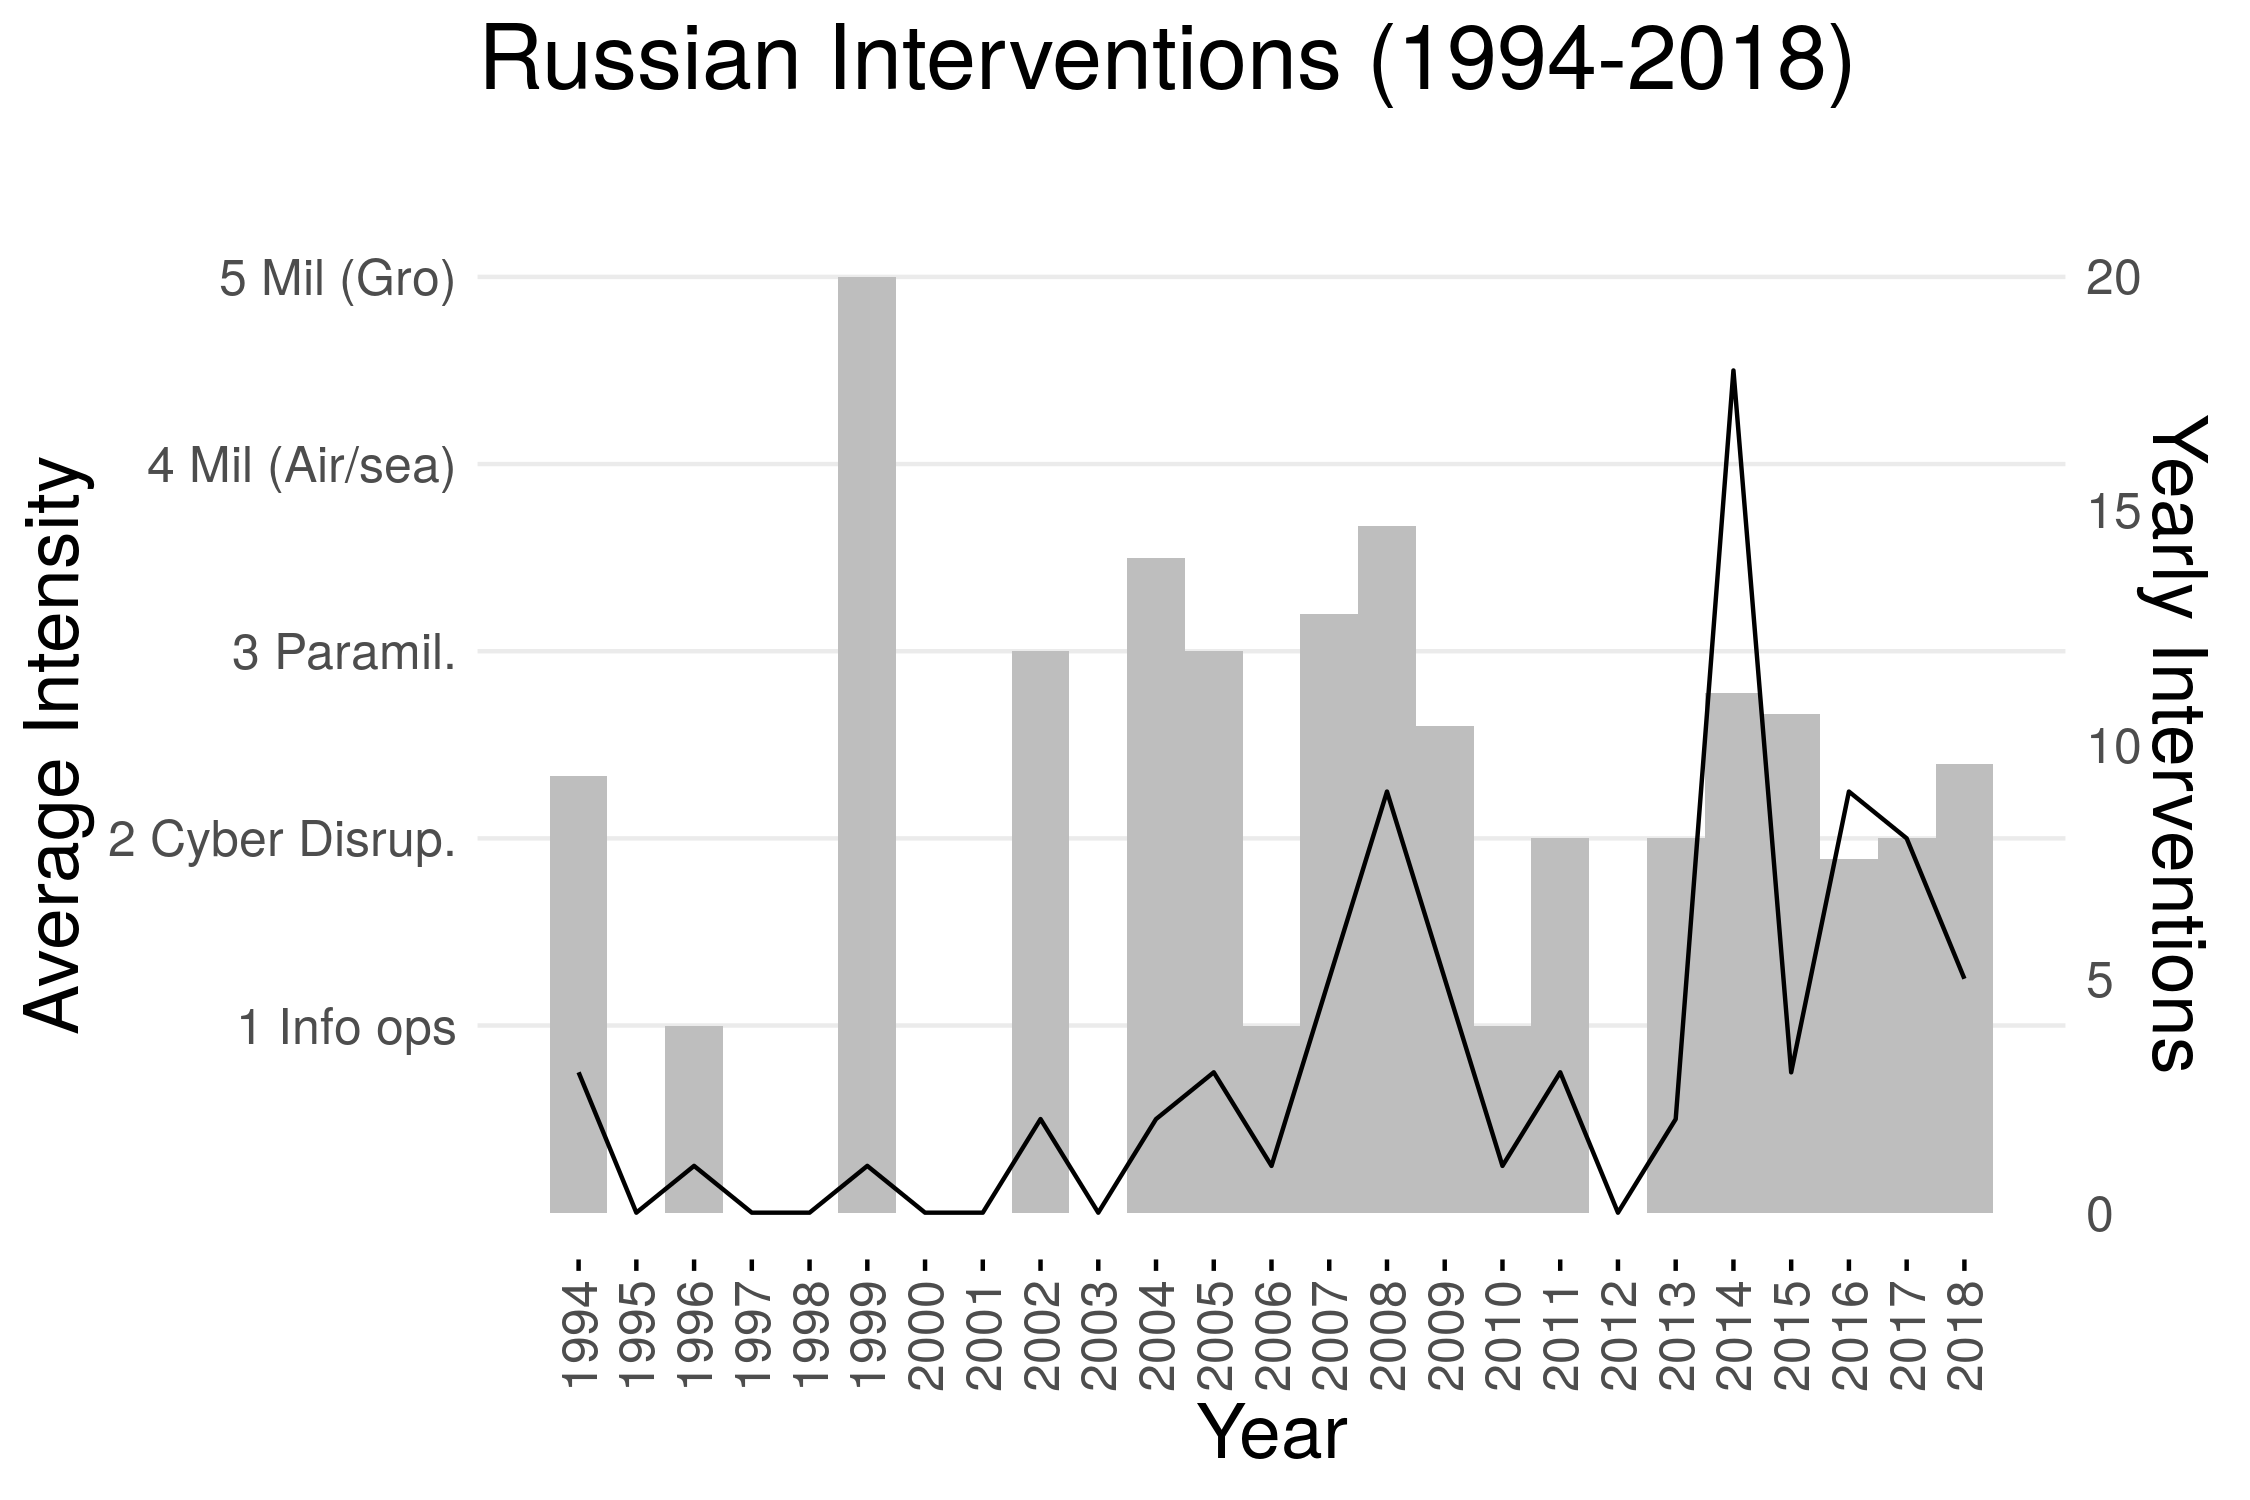
\includegraphics[width = \textwidth]{average_intensity_russian_aggression.png}
		\caption{Intensity of Russian intervention across time. The line represents annual average intensity. Bars denote the number of interventions annually.}
    \label{fig:intensity}
    \end{figure}

Figure \ref{fig:map} depicts a pattern of the geographical coverage of Russian conflict events in Europe. Russia appears to be willing to use more force in countries in its ``near abroad,'' relative to countries further away. Interpreting this geographic pattern on its own is difficult
and highlights the need for more sophisticated analysis.

	\begin{figure}[H]
		\centering
		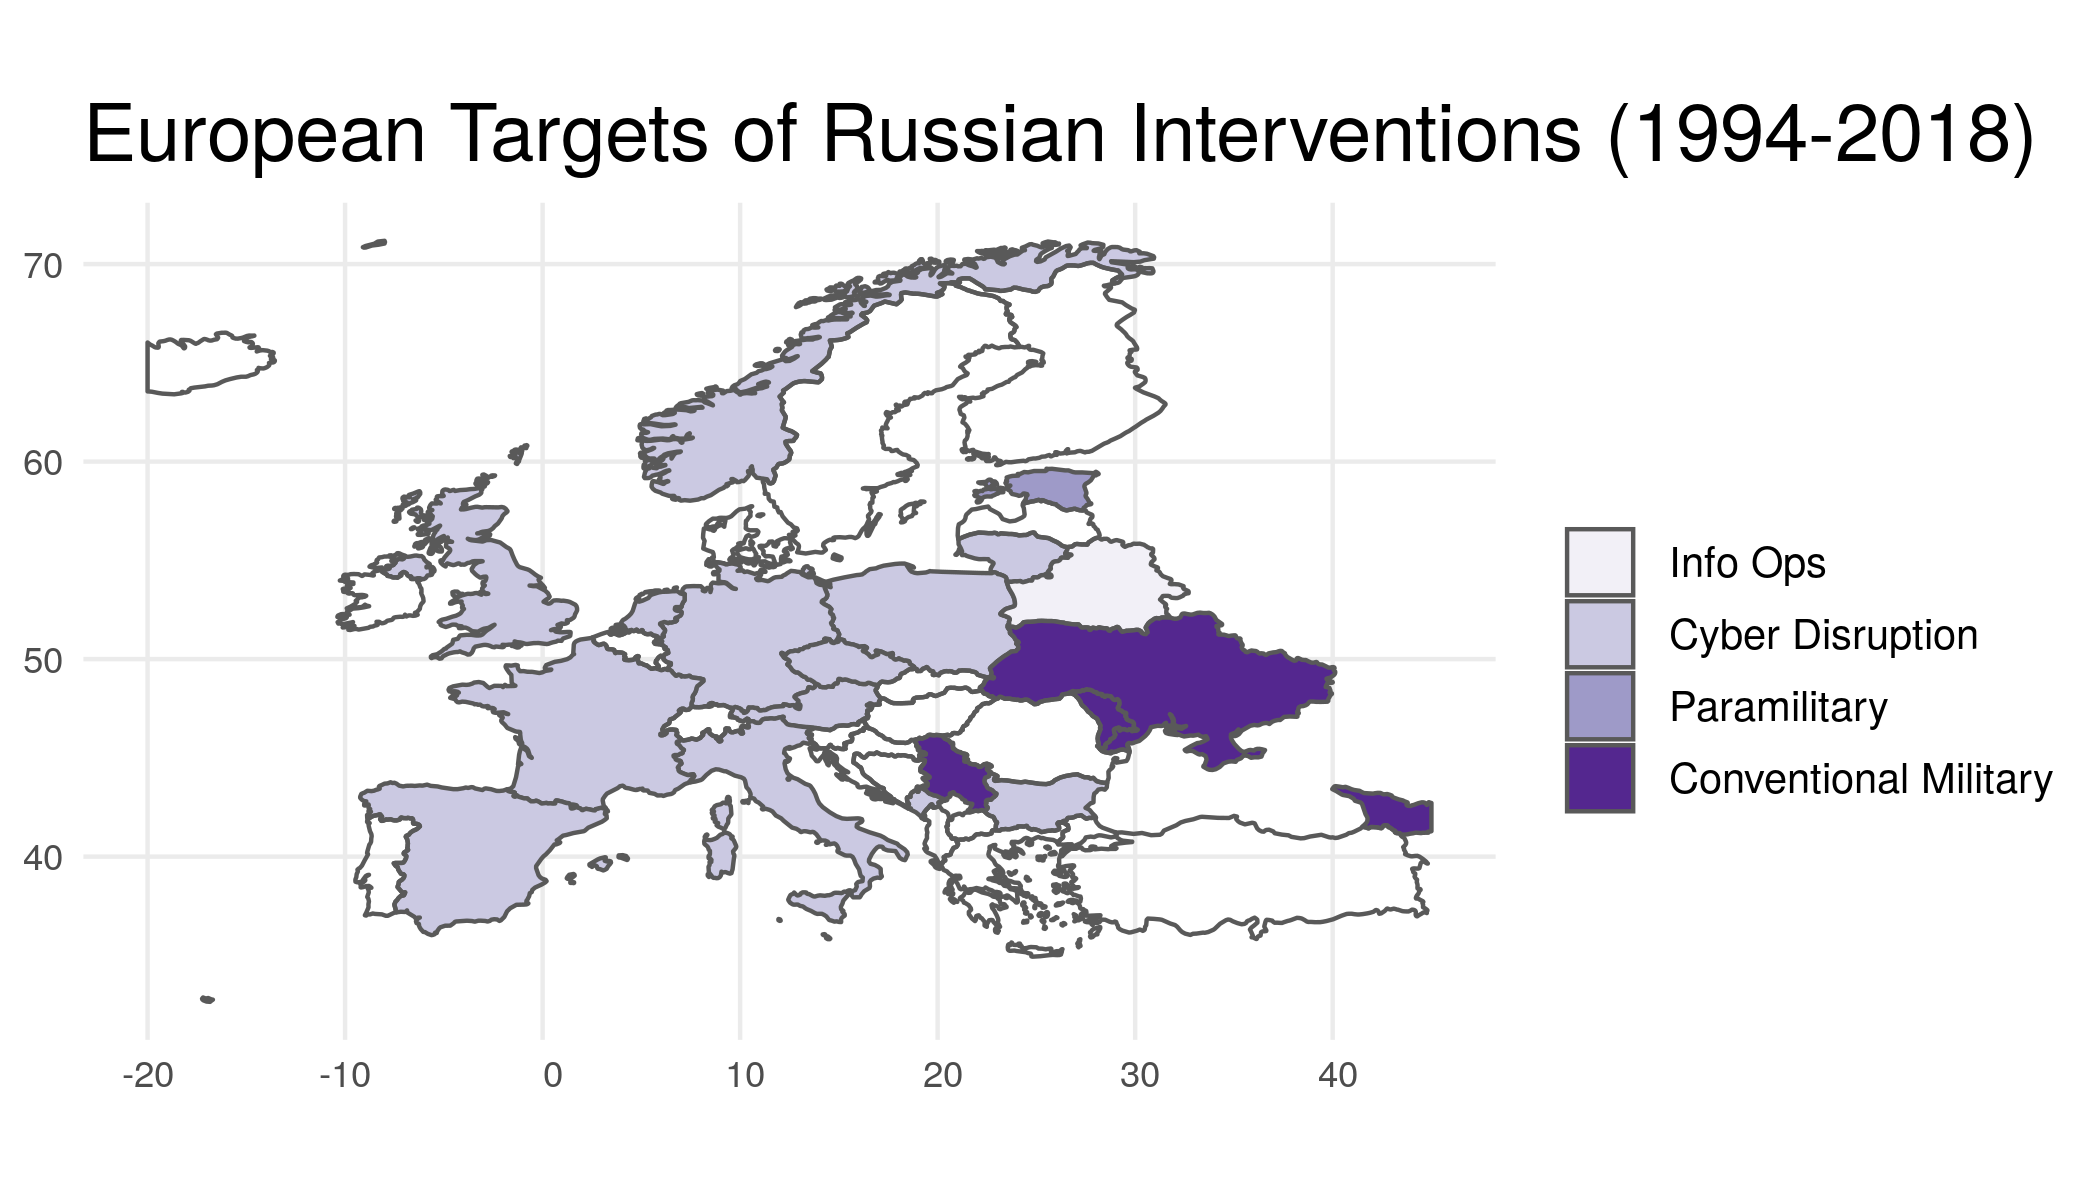
\includegraphics[width = \textwidth]{map_aggregate_europe.png}
		\caption{Geographic representation of Russia intervention. Shading represents the highest intensity of Russian intervention in each European state.}
		\label{fig:map}
	\end{figure}

Now we discuss our independent variables. Consistent with the discussion on the external deterrent threat (Observation 1), we propose that NATO's willingness (or unwillingness) to fight critically shapes Russian gray zone behavior. We operationalize this concept through a dummy variable for NATO membership. NATO members plausibly possess lower costs for fighting since they can rely on collective security, meaning they may possess a reduced willingness to tolerate aggressive low-level behavior from Russia. If Russia is responding to NATO's deterrent threat, we expect NATO states to experience less intense Russian activity.

Consistent with the discussion of the internal-efficiency constraint in Observations 3 and 5, insofar as military power is affected by a loss of strength gradient \citep{posen_commandcommonsmilitary_2003}, Russian gray zone operations will decrease as Russia has less resolve over the issue or faces greater costs for conducting operations when the internal efficiency constraint binds.\footnote{We only analyze this variable in models that also include a NATO membership covariate.} We operationalize Russian resolve and gray zone efficacy jointly through a variable of the logged minimum distance between Russia and each potential-target state, as we expect Russia to care more about states on its periphery and to more easily conduct operations in its proximity \citep{weidmann_geographyinternationalsystem_2010}.

We also include a series of control variables motivated by existing theories of relationships between the control variables and our dependent and independent variables of interest. We include a democracy dummy for states with a Polity V score greater or equal to 6 to control for potential Russian eagerness to target democracies \citep{early_nuclearweaponsexistential_2018}. A state's possession of nuclear weapons may also alter Russia's calculus about how to pursue aggressive actions, so we include a dummy variable for nuclear states \citep{gartzke_strategicapproachnuclear_2009}. We include GDP per capita and the log of population as larger, richer states could generate more opportunities for Russian interventions, especially cyber interventions \citep{beckley_economicdevelopmentmilitary_2010}. Finally, we include military expenditure since it influences both alliance decisions and the cost of undertaking aggression against an adversary \citep{omitoogun_militaryexpendituredata_2006}. Summary statistics are included in the Appendix.

\subsection{Empirical Model and Results}
Because our outcome is an ordinal value, we estimate a series of ordered probit models with year fixed-effects and standard errors clustered by country. Our unit of analysis is the country-year. We run three empirical models on two samples. On the models, first we estimate the relationship between the intensity of Russian intervention and NATO membership and minimum distance from Russia without any control variables. Second, we re-run the first model while also controlling for the range of variables indicated above. We exclude military spending from the second model because it is missing across the entire panel for countries like Yugoslavia and Bosnia \& Herzegovina. In model 3, we include the military spending variable, thus operationalizing military power using population and military spending. On the samples, our first sample (models (1)-(3)) includes all European states. We define state membership using the Gleditsch and Ward state list and continent location using the World Bank Development Indicator \citep{gleditsch_revisedlistindependent_1999}. This excludes micro-states with less than 250,000 people like Liechtenstein and San Marino. The downside is this sample may include states that are not of interest to Russia and may fall outside the scope of our model (i.e., Luxembourg). To address this, our second sample (models (4)-(6)) of ``relevant European states,'' includes only European states that meet any of the following three criteria: a) targets of a Russian attack from 1945-1993 as identified in the Militarized Interstate Dispute (MID) or International Crisis Behavior (ICB) datasets, b) Former Soviet Union or Warsaw Pact states, or c) states that are contiguous with Russia.


\begin{table}[h]
\begin{center}
\begin{tabular}{l c c c c c c}
\hline
 & \multicolumn{3}{c}{Full sample} & \multicolumn{3}{c}{Relevant states sample} \\
\cline{2-4} \cline{5-7}
 & Model 1 & Model 2 & Model 3 & Model 4 & Model 5 & Model 6 \\
\hline
Independent Variables &               &               &               &             &              &               \\
                      &               &               &               &             &              &               \\
\quad NATO member     & $-0.28$       & $-0.46^{**}$  & $-0.60^{***}$ & $-0.47^{*}$ & $-0.58^{**}$ & $-0.68^{***}$ \\
                      & $(0.22)$      & $(0.20)$      & $(0.22)$      & $(0.26)$    & $(0.26)$     & $(0.25)$      \\
\quad Russia distance & $-0.10^{***}$ & $-0.11^{***}$ & $-0.12^{***}$ & $-0.05$     & $-0.09^{**}$ & $-0.09^{**}$  \\
                      & $(0.04)$      & $(0.03)$      & $(0.03)$      & $(0.04)$    & $(0.04)$     & $(0.04)$      \\
Controls              &               &               &               &             &              &               \\
                      &               &               &               &             &              &               \\
\quad Democracy       &               & $0.16$        & $0.46$        &             & $0.12$       & $0.43$        \\
                      &               & $(0.43)$      & $(0.42)$      &             & $(0.45)$     & $(0.43)$      \\
\quad Nuclear power   &               & $0.93^{**}$   & $0.44$        &             & $0.92^{*}$   & $1.06$        \\
                      &               & $(0.42)$      & $(0.44)$      &             & $(0.48)$     & $(0.82)$      \\
\quad Population      &               & $0.19^{**}$   & $0.14$        &             & $0.16$       & $0.18$        \\
                      &               & $(0.09)$      & $(0.12)$      &             & $(0.10)$     & $(0.13)$      \\
\quad GDP per cap     &               & $-0.01^{**}$  & $-0.02^{**}$  &             & $-0.01$      & $-0.01$       \\
                      &               & $(0.01)$      & $(0.01)$      &             & $(0.01)$     & $(0.01)$      \\
\quad Mil. spending   &               &               & $0.02$        &             &              & $-0.00$       \\
                      &               &               & $(0.01)$      &             &              & $(0.02)$      \\
\hline
Observations          & 1,000         & 921           & 891           & 376         & 373          & 346           \\
\hline
\multicolumn{7}{l}{\scriptsize{All models include year-fixed effects with country-clustered standard errors in parentheses. $^{***}p<0.01$; $^{**}p<0.05$; $^{*}p<0.1$}}
\end{tabular}
\caption{Intensity of Russian Intervention: Ordered Probit Results}
\label{table:model}
\end{center}
\end{table}


Table \ref{table:model} presents the coefficient estimates from the ordered probit regressions run on both samples. The results show that both NATO membership and distance from Russia are associated with a decrease the intensity of Russian intervention against European states. Every model that utilizes control variables (models (2), (3), (5), and (6)) suggests the relationship is statistically significant at least at the 0.05 level.

These results provide evidence, subject to standard endogeneity concerns, that Russian gray zone behavior is shaped by  NATO's deterrent threat. Consistent with Observation 1, when facing NATO members, Russia undertook lower-intensity challenges. For example, model (3) reports a proportional odds ratio coefficient of 0.54 on the NATO dummy.\footnote{A complete table of all odds ratios is provided in the Appendix.} This value means that for relevant NATO states, the odds of a non-cyber, non-information attack (categories 3, 4, or 5) are 46\% lower than the odds of experiencing a cyber attack, an information attack, or no attack. Of course, our findings are also consistent with Russian behavior being shaped by their internal cost-benefit calculations (Observations 3 and 5). Naturally these findings can co-exist, suggesting that Russian motives for the scope of their gray zone conflict vary case-by-case. However, consistent with our earlier discussion, what we observe is consistent with deterrence plausibly playing a role.

Our findings are consistent across a range of alternate samples and modeling specifications detailed in the Appendix. As NATO membership is a somewhat coarse operationalization of external deterrent threat, we run additional models distinguishing between non-NATO members in the NATO accession membership process and those who are not.\footnote{The pre-NATO stages includes membership in Partnership for Peace (PfP), Intensified Dialogue, and Membership Action Plan (MAP). For details on what these entail, see \citet{amara_unfulfilledpromisesimpact_2010}.} Additional models also use distance from the nearest NATO state, as intervening in a state neighboring NATO may contain a higher risk of NATO response than interventions not bordering NATO. Additionally, we re-run the analysis including CINC ratios in place of population and the SIPRI military expenditure data \citep{singer_capabilitydistributionuncertainty_1972}.\footnote{Population and military expenditure are two of the six components that comprise the CINC index.} The results from all these models are consistent with the original model specifications. We also find consistent results when sampling on only country-years that experience an attack, with OLS and ordered logit regression models, and using multiple imputation with additive regression, bootstrapping, and predictive mean matching to replace missing values for control variables thus mitigating concern that the initial results are an artifact of listwise deletion \citep{buuren_flexibleimputationmissing_2012, arel-bundock_whencanmultiple_2018}.

\subsection{Case Studies}
The quantitative analysis can be thought of as a coarse technique for considering empirical trends. For a more fine-grained analysis, we consider three major cyber campaigns attributed to Russia that feature prominently in the cybersecurity literature: Estonia, Georgia, and Ukraine. These cases are typically highlighted as examples of the increasing potential of gray zone conflict, making them a most likely case for the conventional efficiency logic. We follow a most similar case study design in selecting cases that feature cyber attacks by the same contiguous challenger (Russia) but differ in other military instruments employed \citep{bennett_casestudymethods_2007}.\footnote{We include a fourth case study of Russian intervention in the 2016 US election in the appendix.} Additionally, Russia has an interest in all states and could intervene with relative ease. 

There are many potential explanations for Russian aspirations in each instance. Here we set aside Russia's foreign policy formulation and focus instead on geopolitical context and military effectiveness. A summary of the extent of Russian intervention in each case is provided in Table \ref{table:russia}; the columns are ordered geographically, West to East, rather than chronologically to highlight the deterrence gradient. Whereas our quantitative analyses proxy NATO membership and geographical distance for the deterrence gradient, our qualitative analysis allows us to add more nuance by considering relative Russian and Western interests.\footnote{We discuss the complicating dynamics of Ukraine in 2022 in the next section.}
    
	\begin{table}[h]
		\centering
		\begin{tabular}{|c||c|c|c|c|}
		    \hline
            \textbf{Russian Operations} & Estonia (2007) & Ukraine (2014) & Georgia (2008) \\
			\hline
            Conventional Forces  &  &  &  X  \\
			\hline
            Special Operations  &  & X & X \\
			\hline
			Cyber Operations & X & X & X \\
			\hline
	    \end{tabular}
        \caption{Case comparison of Russian gray zone conflicts}
		\label{table:russia}
	\end{table}

\subsubsection{Estonia (2007)}
Estonia is the case with the most restrained Russian aggression. The Baltic states formally joined NATO in 2004 receiving only  muted protests from Moscow. Later in 2007, as Putin's foreign policy took on a more combative tenor, the relocation of a Soviet statue in Tallinn triggered a wave of DDoS attacks targeting Estonian banks and government sites \citep{schmidt_estoniancyberattacks_2013}. A symbolic affront to Russian pride was met with symbolic protest. The attacks were carried out by ``patriotic hackers'' with tacit encouragement from Moscow and constituted one of the most disruptive cyber campaigns witnessed up to this time. Yet no one issued any clear demands or claimed responsibility, the attacks were effectively mitigated, and Estonia did not reinstall the statue.\footnote{In the context of our model, the relocated statue represented a new ``status quo,'' where Estonia could engage in independent, nationalist, possibly anti-Russian policy choices. The Russian cyberattack was a (largely futile) attempt to undermine the Estonian government's ability to behave in this manner.} Estonia’s defense minister considered but ultimately rejected invoking Article V, the collective defense clause of the NATO treaty, instead treating the episode as a domestic law enforcement matter \citep{traynor_russiaaccusedunleashing_2007}. Had Estonia not been a NATO member, this consideration would not even have been a possibility, and Russia might well have chosen to act more aggressively.\footnote{Estonians also may not have felt emboldened to provoke Russia in the first place without NATO protection.} Although counterfactuals for the Estonian case are by definition not observable, the fact that Russia engaged in high intensity aggression against Moldova and Georgia during the 2005 to 2009 period while limiting its attacks against Lithuania, Poland, and the United States to cyber attacks and information operations provides suggestive evidence that Russia was clearly using much less force in cases where the defender was more capable or better protected than in cases where a target was weak and isolated politically. The unsettled legal status of a cyberattack in 2007 both enabled and constrained Russia in this respect \citep{joubert_fiveyearsestonia_2012}. Russia and Estonia each understood that NATO was highly unlikely to retaliate for an ambiguous and plausibly deniable outburst, so long as Russia did not inflict serious harm and the level of aggression remained well below the perceived threshold for an Article V response. Overall, in the Estonian case Russian moves are consistent with a desire to avoid escalation. In the aftermath, Estonia overhauled its cyber defenses and established a NATO cybersecurity center, inhibiting future Russian provocations in the gray zone.

\subsubsection{Georgia (2008)}
Georgia is the case with the most Russian aggression. The NATO Bucharest Summit Declaration in April 2008 announced the potential for a Georgian and Ukrainian pathway to NATO membership. This, alongside Kosovo's declaration of independence, triggered a secession crisis in South Ossetia and Abkhazia. Russia announced that it would unilaterally increase peacekeepers in Abkhazia, and hostilities broke out later that year. Georgia was wracked by DDoS service attacks that were encouraged by Moscow, much like Estonia \citep{deibert_cyclonescyberspaceinformation_2012}. Unlike the Estonia case, Russia also deployed columns of conventional armor, naval bombardments, and special operations forces. This case is often cited as an example of how cyberspace can enhance military cross-domain operations, but even more important was Russia's relatively free hand. Russia chose whatever tools it needed to accomplish its objectives and did not pull its punches \citep{binnendijk_understandingrussianblack_2020}. NATO counteraction in the Caucuses was unlikely because Georgia was deep in Russia's traditional sphere of influence and NATO members were publicly worried about Russia's reaction to Georgia joining NATO's Membership Action Plan (MAP). While Russia’s tactical performance left much to be desired, the mission was a strategic success that ended the conversation about Georgia joining NATO. As \citet[590]{driscoll_friendsthesebrinkmanship_2016} point out, Georgia's location -- with Tbilisi a mere 80 miles from the Russian border -- makes it a security liability in the eyes of many Western leaders. Indeed, the Russian intervention served to clarify the stakes of Western interference in Russia's near abroad.

\subsubsection{Ukraine (2014-2021)}
The case of Ukraine, which has already been glossed above, falls in the middle. Consistent with the logic of NATO's deterrent threat binding, Russian actions in Ukraine (prior to 2022) were more extensive than those in Estonia, but much less than what occurred in Georgia. In eight years of protracted low-level conflict, there occurred neither large-scale combined arms warfare, as in Georgia, nor unrestrained ethnic cleansing \citep{driscoll_socialmediarussian_2020}. Russia could have exerted greater military effort, but instead it emphasized cyber attacks, disinformation campaigns, special operations, and military aid to proxy forces. Even though NATO has no formal commitment to Ukraine, conflict in a country that borders four NATO allies (Poland, Slovakia, Hungary, Romania) is implicitly shaped by the possibility of Western intervention, risking nuclear escalation in the process. As a result, we conjecture that Russia acts circumspectly and relatively ineffectively. Endemic Russian cyberattacks and information operations have had little impact on battlefield events \citep{kostyuk_invisibledigitalfront_2019}. Even as social media manipulation is supposedly a Russian specialty, pro-Kremlin narratives have not taken hold in Western Ukraine \citep{driscoll_socialmediarussian_2020}. By and large, Russian subversion has failed to influence Kyiv (other than pushing it Westward) \citep{maschmeyer_subversivetrilemmawhy_2021}.

\subsubsection{Discussion of Cases}
All three cases, each often cited to exemplify the potency of cyber-enabled gray zone conflict, are consistent with our hypothesis that deterrence encourages capable actors to engage in calculated restraint. As the deterrent threat from NATO becomes more salient moving westward from Georgia to Ukraine and finally to Estonia, Russia pursues its international objectives with lower intensity.

One might argue that Russia has different levels of resolve across these cases. For example, one might argue that Russia places a very different value on the outcome in Ukraine than Estonia. Indeed, Russia let Estonia join NATO without a fight in 2004, and Russia's historical ties with Estonia are weaker. By contrast, Russia had supported Georgian separatists since the early 1990s and was highly resolved to ward off Western encroachment. The comparison of Georgia and Ukraine, however, finds this alternative account wanting. While Georgia may be the birthplace of Stalin, it is also a peripheral outpost in the Caucuses far from Moscow. By contrast, the Black Sea port of Sevastopol makes Crimea strategically important, and NATO forces in Ukraine would be perceived as a dagger pointing at Moscow. The seat of the medieval Kievan Rus empire is also more salient in Russian nationalist mythology than Georgia ever was. If Russian moves were motivated by resolve rather than external deterrence, then we would expect more robust, and more overt, Russian military efforts in Ukraine. Yet, despite Russia’s undoubted higher valuation for the stakes in Ukraine, Russia showed more restraint there for eight years, at least until the February 2022 invasion (as we discuss in the next section).

\section{Gray Zone Efficacy and Escalation Dynamics}\label{counterintuitivefinding}

\label{gzdefense} Beyond microfounding the motives for gray zone conflict behavior, our model can also offer insight into an important policy question: how can a defender best react to the prospect of gray zone conflict? 

It might seem intuitive that improvements in a defender's capacity to counter gray zone aggression should reinforce the strength of deterrence, but this is not necessarily the case. As the defender becomes more capable at gray zone conflict (here approximated by lowering $\beta_{D}$), this constrains how productive gray zone conflict can be for the challenger. And, as the gray zone conflict option becomes worse for the challenger, the challenger will consider other policy options; sometimes the defender getting better at gray zone conflict will effectively deter the challenger---convince the challenger not to challenge and accept the ``status quo''---but other times this change will encourage the challenger to behave more aggressively and risk a war. In terms of the risk-return trade-off discussed in Section \ref{risk_return}, consider a scenario where, in equilibrium, the challenger is choosing a conservative challenge that always results in gray zone conflict.\footnote{Formally, C is choosing $g_{C}^{*}=g_{C}^{GZ,EDT}$ or $g_{C}^{*}=g_{C}^{GZ,IE}$.} This means the challenger is not choosing a more aggressive challenge that would sometimes result in (a more productive form of) gray zone conflict and would sometimes result in war.\footnote{Formally, C is not choosing $g_{C}^{*}=g_{C}^{W,EDT}$ or $g_{C}^{*}=g_{C}^{W,IE}$.} As the defender becomes better at gray zone conflict, gray zone conflict becomes less beneficial for the challenger; all the while, the challenger's war payoffs remain the same. This means that the ``downside'' of a more aggressive challenge---the game ending in war---does not look as bad to the challenger given that the challenger is now doing worse playing it safe.

This intuition can be visualized in Figure \ref{bettergzc}. The basic logic for why this figure looks as it does is described in Section \ref{risk_return}, but it is worthwhile highlighting the value $\theta\rho-\kappa_C$ on the y-axis, which is C's expected payoff should the game end in war. In the top panel, when $\beta_{D}=5$, C attains the greatest payoff setting $g_{C}^{*}=g_{C}^{GZ,EDT}$ and never risking war. It is worthwhile noting what C is not doing. C could risk war from setting $g_{C}=g_{C}^{W,EDT}$, which would result in a greater payoff if the game ends in gray zone conflict (when D is type $\bar{\kappa}_{D}$), but would also result in a much lower payoff if the game ends in war (when D is type $\underline{\kappa}_{D}$). Here, the downside of C setting $g_{C}=g_{C}^{W,EDT}$ and risking war---C having to fight a war---is so much worse than C's payoff of playing it safe and setting $g_{C}=g_{C}^{GZ,EDT}$, that C will not take the risk and will optimally set$g_{C}^{*}=g_{C}^{GZ,EDT}$.

\begin{figure}  

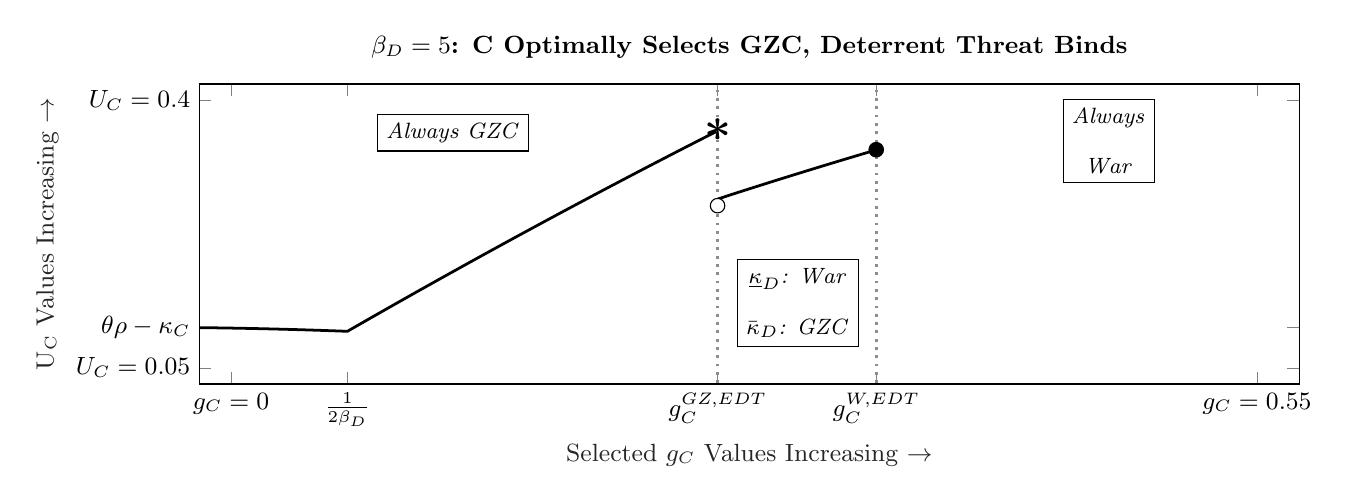
\begin{tikzpicture} 
\small
\begin{axis}[%
width=5.5in,
height=1.5in,
at={(1.011in,0.642in)},
scale only axis,
xmin=0.03,
xmax=0.55,
xtick={0.045,0.1, 0.275,0.35, 0.53},
xticklabels={{$g_C=0$},{$\frac{1}{2\beta_D}$},{$g_{C}^{GZ,EDT}$},{$g_{C}^{W,EDT}$},{$g_C=0.55$}},
xlabel style={font=\color{white!15!black}},
xlabel={Selected $g_C$ Values Increasing $\rightarrow$},
ymin=0.05,
ymax=0.42,
ytick={0.07,0.12,0.4},
yticklabels={{$U_C=0.05$},{$ \theta\rho-\kappa_C$},{$U_C=0.4$}},
ylabel style={font=\color{white!15!black}},
ylabel={$\text{U}_\text{C}$ Values Increasing $\rightarrow$},
axis background/.style={fill=white},
title style={font=\bfseries},
title={$\beta_D=5$: C Optimally Selects GZC, Deterrent Threat Binds},
]

\node[draw, align=center] at (0.15,0.36) {\footnotesize{\textit{Always GZC}}}; 

\node[draw, align=center] at (0.313,0.15) {\footnotesize{\textit{$\underline{\kappa}_D$: War}} \\\footnotesize{\textit{$\bar{\kappa}_D$: GZC}}}; 

\node[draw, align=center] at (0.46,0.35) {\footnotesize{\textit{Always}} \\\footnotesize{\textit{War}}}; 


\addplot [color=black, line width=1.0pt]
  table[row sep=crcr]{%
0	0.12	\\
0.005	0.1199875	\\
0.01	0.11995	\\
0.015	0.1198875	\\
0.02	0.1198	\\
0.025	0.1196875	\\
0.03	0.11955	\\
0.035	0.1193875	\\
0.04	0.1192	\\
0.045	0.1189875	\\
0.05	0.11875	\\
0.055	0.1184875	\\
0.06	0.1182	\\
0.065	0.1178875	\\
0.07	0.11755	\\
0.075	0.1171875	\\
0.08	0.1168	\\
0.085	0.1163875	\\
0.09	0.11595	\\
0.095	0.1154875	\\
0.1	0.115	\\
0.105	0.1224875	\\
0.11	0.12995	\\
0.115	0.1373875	\\
0.12	0.1448	\\
0.125	0.1521875	\\
0.13	0.15955	\\
0.135	0.1668875	\\
0.14	0.1742	\\
0.145	0.1814875	\\
0.15	0.18875	\\
0.155	0.1959875	\\
0.16	0.2032	\\
0.165	0.2103875	\\
0.17	0.21755	\\
0.175	0.2246875	\\
0.18	0.2318	\\
0.185	0.2388875	\\
0.19	0.24595	\\
0.195	0.2529875	\\
0.2	0.26	\\
0.205	0.2669875	\\
0.21	0.27395	\\
0.215	0.2808875	\\
0.22	0.2878	\\
0.225	0.2946875	\\
0.23	0.30155	\\
0.235	0.3083875	\\
0.24	0.3152	\\
0.245	0.3219875	\\
0.25	0.32875	\\
0.255	0.3354875	\\
0.26	0.3422	\\
0.265	0.3488875	\\
0.27	0.35555	\\
0.275	0.3621875	\\
};


\addplot [color=black, line width=1.0pt]
  table[row sep=crcr]{%
0.275	0.278	\\
0.28	0.2824	\\
0.285	0.2865875	\\
0.29	0.29075	\\
0.295	0.2948875	\\
0.3	0.299	\\
0.305	0.3030875	\\
0.31	0.30715	\\
0.315	0.3111875	\\
0.32	0.3152	\\
0.325	0.3191875	\\
0.33	0.32315	\\
0.335	0.3270875	\\
0.34	0.331	\\
0.345	0.3348875	\\
0.35	0.33875	\\
};



\addplot [color=white!55!black, dotted, line width=1.0pt, forget plot]
  table[row sep=crcr]{%
0.275	0\\
0.275	1.5\\
};

\addplot [color=white!55!black, dotted, line width=1.0pt, forget plot]
  table[row sep=crcr]{%
0.35	0\\
0.35	1.5\\
};


\node at (0.275,0.355) {\LARGE \textbf{*}};
\node at (0.275,0.27) [circle,scale=0.6,draw,fill=black!0] {};
\node at (0.35,0.339) [circle,scale=0.6,minimum size=0.5pt,draw,fill=black!100] {};
%\node at (0.503,0.53) [circle,scale=0.6,minimum size=0.5pt,draw,fill=black!100] {};
            

\end{axis}
\end{tikzpicture} \vspace{.6cm}


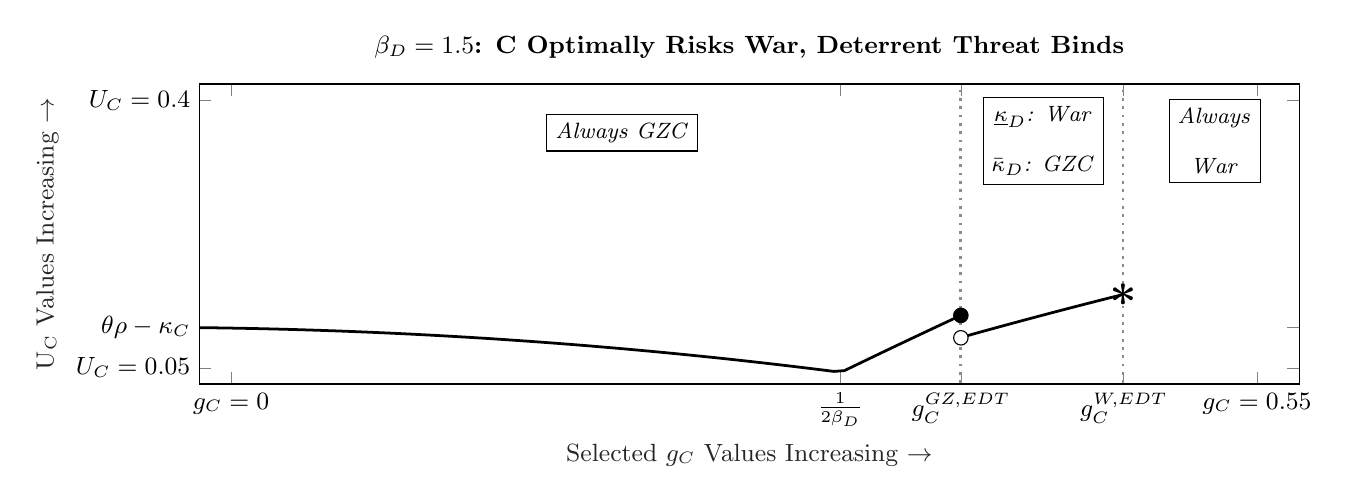
\begin{tikzpicture} 
\small
\begin{axis}[%
width=5.5in,
height=1.5in,
at={(1.011in,0.642in)},
scale only axis,
xmin=0.03,
xmax=0.55,
xtick={0.045,0.333, 0.39,0.467, 0.53},
xticklabels={{$g_C=0$},{$\frac{1}{2\beta_D}$},{$g_{C}^{GZ,EDT}$},{$g_{C}^{W,EDT}$},{$g_C=0.55$}},
xlabel style={font=\color{white!15!black}},
xlabel={Selected $g_C$ Values Increasing $\rightarrow$},
ymin=0.05,
ymax=0.42,
ytick={0.07,0.12,0.4},
yticklabels={{$U_C=0.05$},{$ \theta\rho-\kappa_C$},{$U_C=0.4$}},
ylabel style={font=\color{white!15!black}},
ylabel={$\text{U}_\text{C}$ Values Increasing $\rightarrow$},
axis background/.style={fill=white},
title style={font=\bfseries},
title={$\beta_D=1.5$: C Optimally Risks War, Deterrent Threat Binds},
]

\node[draw, align=center] at (0.23,0.36) {\footnotesize{\textit{Always GZC}}}; 

\node[draw, align=center] at (0.429,0.35) {\footnotesize{\textit{$\underline{\kappa}_D$: War}} \\\footnotesize{\textit{$\bar{\kappa}_D$: GZC}}}; 

\node[draw, align=center] at (0.51,0.35) {\footnotesize{\textit{Always}} \\\footnotesize{\textit{War}}}; 


\addplot [color=black, line width=1.0pt]
  table[row sep=crcr]{%
0	0.12	\\
0.005	0.1199875	\\
0.01	0.11995	\\
0.015	0.1198875	\\
0.02	0.1198	\\
0.025	0.1196875	\\
0.03	0.11955	\\
0.035	0.1193875	\\
0.04	0.1192	\\
0.045	0.1189875	\\
0.05	0.11875	\\
0.055	0.1184875	\\
0.06	0.1182	\\
0.065	0.1178875	\\
0.07	0.11755	\\
0.075	0.1171875	\\
0.08	0.1168	\\
0.085	0.1163875	\\
0.09	0.11595	\\
0.095	0.1154875	\\
0.1	0.115	\\
0.105	0.1144875	\\
0.11	0.11395	\\
0.115	0.1133875	\\
0.12	0.1128	\\
0.125	0.1121875	\\
0.13	0.11155	\\
0.135	0.1108875	\\
0.14	0.1102	\\
0.145	0.1094875	\\
0.15	0.10875	\\
0.155	0.1079875	\\
0.16	0.1072	\\
0.165	0.1063875	\\
0.17	0.10555	\\
0.175	0.1046875	\\
0.18	0.1038	\\
0.185	0.1028875	\\
0.19	0.10195	\\
0.195	0.1009875	\\
0.2	0.1	\\
0.205	0.0989875	\\
0.21	0.09795	\\
0.215	0.0968875	\\
0.22	0.0958	\\
0.225	0.0946875	\\
0.23	0.09355	\\
0.235	0.0923875	\\
0.24	0.0912	\\
0.245	0.0899875	\\
0.25	0.08875	\\
0.255	0.0874875	\\
0.26	0.0862	\\
0.265	0.0848875	\\
0.27	0.08355	\\
0.275	0.0821875	\\
0.28	0.0808	\\
0.285	0.0793875	\\
0.29	0.07795	\\
0.295	0.0764875	\\
0.3	0.075	\\
0.305	0.0734875	\\
0.31	0.07195	\\
0.315	0.0703875	\\
0.32	0.0688	\\
0.325	0.0671875	\\
0.33	0.06555	\\
0.335	0.066554167	\\
0.34	0.072866667	\\
0.345	0.079154167	\\
0.35	0.085416667	\\
0.355	0.091654167	\\
0.36	0.097866667	\\
0.365	0.104054167	\\
0.37	0.110216667	\\
0.375	0.116354167	\\
0.38	0.122466667	\\
0.385	0.128554167	\\
0.39	0.134616667	\\
};


\addplot [color=black, line width=1.0pt]
  table[row sep=crcr]{%
0.39	0.107	\\
0.395	0.111054167	\\
0.4	0.114666667	\\
0.405	0.118254167	\\
0.41	0.121816667	\\
0.415	0.125354167	\\
0.42	0.128866667	\\
0.425	0.132354167	\\
0.43	0.135816667	\\
0.435	0.139254167	\\
0.44	0.142666667	\\
0.445	0.146054167	\\
0.45	0.149416667	\\
0.455	0.152754167	\\
0.46	0.156066667	\\
0.465	0.159354167	\\
0.4667	0.1604	\\
};




%\addplot [color=white!55!black, dotted, line width=1.0pt, forget plot]
%  table[row sep=crcr]{%
%0.1	-1\\
%0.1	1\\
%};


\addplot [color=white!55!black, dotted, line width=1.0pt, forget plot]
  table[row sep=crcr]{%
0.39	0\\
0.39	1.5\\
};

\addplot [color=white!55!black, dotted, line width=1.0pt, forget plot]
  table[row sep=crcr]{%
0.4667	0\\
0.4667	1.5\\
};


\node at (0.4667,0.152) {\LARGE \textbf{*}};
\node at (0.39,	0.107) [circle,scale=0.6,draw,fill=black!0] {};
\node at (0.39,	0.134616667) [circle,scale=0.6,minimum size=0.5pt,draw,fill=black!100] {};
%\node at (0.503,0.53) [circle,scale=0.6,minimum size=0.5pt,draw,fill=black!100] {};
            

\end{axis}
\end{tikzpicture} 

\caption{C's Utility Across selected $g_C$'s.}\label{bettergzc}
\caption*{ C's optimal $g_C$ is marked by the asterisks. The regions denote how D responds to a selected $g_C$---whether D will always engage with a gray zone response, whether D will always go to war, or whether different types of D respond differently. All sub-figures have the same underlying parameters (listed in the Appendix), except $\beta_C$ which varies across sub-figures.}
\end{figure}

In the bottom panel, when $\beta_{D}=1.5$, C now does best setting $g_{C}=g_{C}^{W,EDT}$ and sometimes risking war. Why? As D becomes better at gray zone conflict, C does worse within all gray zone conflict outcomes. Visually, under $\beta_{D}=1.5$, C setting $g_{C}=g_{C}^{GZ,EDT}$ is now much worse for C. So much worse, in fact, that the downside of C risking war---C's wartime payoff of $ \theta\rho-\kappa_C$---is only slightly less than C's payoff from setting $g_{C}=g_{C}^{GZ,EDT}$. Here, as $\beta_{D}$ decreases, C does so poorly in gray zone conflict that now war does not look nearly as bad; this can incentivize C to tolerate the downside risk of war in order to attain a greater ``upside'' of a more aggressive gray zone challenge.

Note that the discussion above does not claim that decreases in the defender's gray zone costs always leads to war. As D gets better at gray zone conflict, C could instead be pressured out of challenging altogether and instead accept the status quo. A key factor that determines whether decreases in $\beta_{D}$ result in C switching from gray zone conflict to war or peace is C's resolve. When the challenger possess a high resolve, a decrease in $\beta_{D}$ will result in war under more circumstances. These finding can be summarized in Observation 7.

\textbf{\textit{Observation 7:}}\textit{ Decreases in the defender's gray zone costs ($\beta_{D}$) can lead to war, especially when C's resolve ($\theta$) is high.}

Until this point, we have discussed $\beta_{D}$ as the defender's gray zone capabilities stemming from technological capabilities. There is an alternate interpretation as well; $\beta_{D}$ could be influenced by the defender's prior, un-modeled moves in the game that set up current gray zone operations. For example, if the defender aggressively pursued counterinsurgency operations against foreign-backed rebels before this game began, the defender could be in a better position to pursue aggressive gray zone conflict within the game. This interpretation illustrates how it is not just latent, exogenous costs that influence the challenger's activity. Rather, war can result from the defender behaving too aggressively in prior gray actions against a highly resolved challenger.

This final interpretation has important policy consequences being played-out in Ukraine since February 2022. After roughly eight years of gray zone conflict in Ukraine, Russia dramatically changed course by invading Ukraine, thus initiating a highly aggressive war. This escalation raises an important question about gray zone conflict: why, if subversion is such an efficient way of revising the status quo without triggering open war, would Russia choose to accept the costs and risks of threatening just such a war? Our research poses one answer to this question. Over the past eight years, through internal improvements and external support, Ukraine has gotten better at fighting in the gray zone, which has made gray zone untenable for Russia. Our model suggests there could be a connection between improved Ukrainian gray zone capabilities (2014-2021) and the Russian escalation that followed. Of course, we cannot say for certain that this element drove Russia escalation; it is exceptionally difficult to identify what drives international decision making. For example, it could be that Russia came to view itself as more of a declining power in the lead up to the 2022 invasion, perhaps due to arms transfers to Ukraine or the warming relations between NATO and Ukraine \citep{benson_commitmentproblemsalliance_2022}. However, even if we are incorrect in this one case, our model still suggests an important implication for future policy: challengers with high resolve, when faced with worse options within the gray zone conflict policy space, may seek more aggressive means of conducting international politics. 

There are three additional technical points worth mentioning. First, further discussion on this result, details on Observation 7, and comparative statics are found in the Appendix (Section 1.8). Second, reasonable readers might be concerned that the results are driven entirely by $\beta_{D}$ not altering war payoffs. In the Appendix, we demonstrate a similar result to Observation 7 for a model where, as D gets better at gray zone conflict, D also gets better at war and C also gets worse at war. While the results are more complex and notation-heavy, the general mechanism remains (though with some limits). Third, a result like Observation 7 can also exist in a model where commitment problems (rather than incomplete information) are drivers of war. We explore this in Appendix Section 3.

\section{Every Silver Lining's Got a Touch of Gray}
Gray zone conflict occurs when capable actors intentionally limit the intensity or capacity of aggression and refrain from escalation. Deterrence shapes the way that conflict emerges, but it may not suppress conflict altogether. The good news is that gray zone conflict may be symptomatic of deterrence success. Adversaries could be “designing around” deterrence in an effort to avoid the anticipated retaliation of the defender \citep{lieberman_reconceptualizingdeterrencenudging_2012}. The bad news is that gray zone conflict probes the threshold of deterrence effectiveness. We expect conflict severity to be greater wherever there are questions about the willingness or ability of defenders to respond forcefully. An adversary is seldom passive. There will always be attempts at end-runs or push-back, even when deterrence is credible. It is thus important to think carefully before overextending commitments where credibility is in doubt. 

Just as there is a gray zone between war and peace, the distinction between effective and ineffective deterrence is also fuzzy. Doubling down on deterrence in the gray zone can mitigate conflict in some cases but provoke escalation in the others. Wherever deterrence is credible, or the challenger's resolve is low, challengers can be expected to exercise restraint as they probe to see what they can get away with. Wherever deterrence is not credible or challengers are highly resolved, however, a challenger will be more emboldened to use whatever means they have at their disposal to meet their objectives, limited only by internal efficiency constraints.

We have used the same cases that have raised alarm about the dangers of gray zone conflict to suggest the validity of an alternative explanation. The evidence suggests that Russia may systematically reduce the intensity of its interventions due to deterrence, employing a greater variety of means with more lethal intensity where deterrence is weakest but conducting only ambiguous information operations where deterrence is most robust. The conventional wisdom is right that Russian interventions are paradigmatic exemplars of gray zone conflict, but it is wrong about Russian motivations and the effectiveness of these operations. Revisionist powers have not discovered a secret formula or novel tools destined to destabilize Western democracies or undermine NATO's deterrence posture. Rather it acts opportunistically as circumstances enable it to hassle adversaries and their clients without risking a costly military confrontation. The flip side of this logic, however, is that Russia is willing to call NATO’s bluffs in cases where it can reasonably expect that NATO is unwilling to intervene. In Georgia, and even more so in Chechnya, Russian willingness to prioritize effectiveness at the price of efficiency is clear. Ukraine after 2021 provides a more nuanced, and more dangerous, illustration of this general logic.

The very fact that an adversary opts to engage in limited conflict suggests both vulnerabilities and opportunities. Instead of worrying about Western paralysis in response to Russian cunning, we can acknowledge that NATO has already blocked Russia from wielding even greater influence. NATO's implicit general deterrence posture has arguably succeeded in keeping more extreme forms of Russian aggression in check. The unfortunate fact remains, however, that a simple remedy for gray zone conflict does not exist, if only because there is always some ability to ``design around''  deterrence. We may be able to choose \textit{how} our adversary confronts us, but not \textit{whether}. Deterrence is not an on/off switch, but a rheostat, providing a range of causes and variable effects. Gray zone conflict is, then, not simply deterrence failure but also a modest kind of success.

\newpage

\bibliography{GrayZone.bib}

\end{document}